\ifx\allfiles\undefined
\documentclass[12pt, a4paper,oneside, UTF8]{ctexbook}
\usepackage[dvipsnames]{xcolor}
\usepackage{mathtools}   % 数学公式(mathtools 是 amsmath 的上位替代)
\usepackage{amsthm}    % 定理环境
\usepackage{amssymb}   % 更多公式符号
\usepackage{graphicx}  % 插图
%\usepackage{mathrsfs}  % 数学字体
%\usepackage{newtxtext,newtxmath}
%\usepackage{arev}
\usepackage{kmath,kerkis}
\usepackage{newtxtext}
\usepackage{bbm}
\usepackage{enumitem}  % 列表
\usepackage{geometry}  % 页面调整
%\usepackage{unicode-math}
\usepackage[colorlinks,linkcolor=black]{hyperref}

\usepackage{wrapfig}


\usepackage{ulem}	   % 用于更多的下划线格式,
					   % \uline{}下划线,\uuline{}双下划线,\uwave{}下划波浪线,\sout{}中间删除线,\xout{}斜删除线
					   % \dashuline{}下划虚线,\dotuline{}文字底部加点


\graphicspath{ {flg/},{../flg/}, {config/}, {../config/} }  % 配置图形文件检索目录
\linespread{1.5} % 行高

% 页码设置
\geometry{top=25.4mm,bottom=25.4mm,left=20mm,right=20mm,headheight=2.17cm,headsep=4mm,footskip=12mm}

% 设置列表环境的上下间距
\setenumerate[1]{itemsep=5pt,partopsep=0pt,parsep=\parskip,topsep=5pt}
\setitemize[1]{itemsep=5pt,partopsep=0pt,parsep=\parskip,topsep=5pt}
\setdescription{itemsep=5pt,partopsep=0pt,parsep=\parskip,topsep=5pt}

% 定理环境
% ########## 定理环境 start ####################################
\theoremstyle{definition}
\newtheorem{defn}{\indent 定义}[section]

\newtheorem{lemma}{\indent 引理}[section]    % 引理 定理 推论 准则 共用一个编号计数
\newtheorem{thm}[lemma]{\indent 定理}
\newtheorem{corollary}[lemma]{\indent 推论}
\newtheorem{criterion}[lemma]{\indent 准则}

\newtheorem{proposition}{\indent 命题}[section]
\newtheorem{example}{\indent \color{SeaGreen}{例}}[section] % 绿色文字的 例 ,不需要就去除\color{SeaGreen}{}
\newtheorem*{rmk}{\indent \color{red}{注}}

% 两种方式定义中文的 证明 和 解 的环境:
% 缺点:\qedhere 命令将会失效【技术有限,暂时无法解决】
\renewenvironment{proof}{\par\textbf{证明.}\;}{\qed\par}
\newenvironment{solution}{\par{\textbf{解.}}\;}{\qed\par}

% 缺点:\bf 是过时命令,可以用 textb f等替代,但编译会有关于字体的警告,不过不影响使用【技术有限,暂时无法解决】
%\renewcommand{\proofname}{\indent\bf 证明}
%\newenvironment{solution}{\begin{proof}[\indent\bf 解]}{\end{proof}}
% ######### 定理环境 end  #####################################

% ↓↓↓↓↓↓↓↓↓↓↓↓↓↓↓↓↓ 以下是自定义的命令  ↓↓↓↓↓↓↓↓↓↓↓↓↓↓↓↓

% 用于调整表格的高度  使用 \hline\xrowht{25pt}
\newcommand{\xrowht}[2][0]{\addstackgap[.5\dimexpr#2\relax]{\vphantom{#1}}}

% 表格环境内长内容换行
\newcommand{\tabincell}[2]{\begin{tabular}{@{}#1@{}}#2\end{tabular}}

% 使用\linespread{1.5} 之后 cases 环境的行高也会改变,重新定义一个 ca 环境可以自动控制 cases 环境行高
\newenvironment{ca}[1][1]{\linespread{#1} \selectfont \begin{cases}}{\end{cases}}
% 和上面一样
\newenvironment{vx}[1][1]{\linespread{#1} \selectfont \begin{vmatrix}}{\end{vmatrix}}

\def\d{\textup{d}} % 直立体 d 用于微分符号 dx
\def\R{\mathbb{R}} % 实数域
\def\N{\mathbb{N}} % 自然数域
\def\C{\mathbb{C}} % 复数域
\def\Z{\mathbb{Z}} % 整数环
\def\Q{\mathbb{Q}} % 有理数域
\newcommand{\bs}[1]{\boldsymbol{#1}}    % 加粗,常用于向量
\newcommand{\ora}[1]{\overrightarrow{#1}} % 向量

% 数学 平行 符号
\newcommand{\pll}{\kern 0.56em/\kern -0.8em /\kern 0.56em}

% 用于空行\myspace{1} 表示空一行 填 2 表示空两行  
\newcommand{\myspace}[1]{\par\vspace{#1\baselineskip}}

%s.t. 用\st就能打出s.t.
\DeclareMathOperator{\st}{s.t.}

%罗马数字 \rmnum{}是小写罗马数字, \Rmnum{}是大写罗马数字
\makeatletter
\newcommand{\rmnum}[1]{\romannumeral #1}
\newcommand{\Rmnum}[1]{\expandafter@slowromancap\romannumeral #1@}
\makeatother
\begin{document}
	% \title{{\Huge{\textbf{$Partial \,\, Differential \,\, Equations$}}}\footnote{参考书籍:\\
			\hspace*{4em} \textbf{《Partial Differential Equations》 -- Lawrence C. Evans} \\
			\hspace*{4em} \textbf{《Partial Differential Equations》 -- Fritz John} \\
			\hspace*{4em} \textbf{《数学物理方程讲义 (第二版)》--  姜礼尚、陈亚浙、刘西垣、易法槐} 
			}}
\author{$-TW-$}
\date{\today}
\maketitle                   % 在单独的标题页上生成一个标题

\thispagestyle{empty}        % 前言页面不使用页码
\begin{center}
	\Huge\textbf{序}
\end{center}


\vspace*{3em}
\begin{center}
	\large{\textbf{天道几何,万品流形先自守;}}\\
	
	\large{\textbf{变分无限,孤心测度有同伦。}}
\end{center}

\vspace*{3em}
\begin{flushright}
	\begin{tabular}{c}
		\today \\ \small{\textbf{长夜伴浪破晓梦,梦晓破浪伴夜长}}
	\end{tabular}
\end{flushright}


\newpage                      % 新的一页
\pagestyle{plain}             % 设置页眉和页脚的排版方式(plain:页眉是空的,页脚只包含一个居中的页码)
\setcounter{page}{1}          % 重新定义页码从第一页开始
\pagenumbering{Roman}         % 使用大写的罗马数字作为页码
\tableofcontents              % 生成目录

\newpage                      % 以下是正文
\pagestyle{plain}
\setcounter{page}{1}          % 使用阿拉伯数字作为页码
\pagenumbering{arabic}
\setcounter{chapter}{0}    % 设置 -1 可作为第零章绪论从第零章开始 
	\else
	\fi
	%  ############################ 正文部分
\chapter{Second-Order Equations : Hyperbolic Equations for Functions of Two Variables}

	这一章我们来讨论\textbf{含2个自变量的2阶PDE}, 首先将\textbf{特征线}的推广至2阶Quasi-Linear Equation上, 并利用特征线来对\textbf{2阶Linear Equation}进行化简分类, 而后我们将重点讨论\textbf{一维波动方程}, 介绍其两种不同的解法. 

\section{Characteristics for Quasi-Linear Second-Order Equations}
	这一节我们将讨论一般的\textbf{含2个自变量的2阶Quasi-Linear Equation的Cauchy问题}, 讨论其解的存在性问题, 并引出\textbf{特征线}的拓展定义, 为后续\textbf{Linear Equation} 的化简分类工作做好铺垫. 

	\vspace*{2em}

	\hspace*{-1.85em}Consider the general Quasi-Linear Equation
	\begin{align}
		au_{xx} + 2b u_{xy} + c u_{yy} = d \label{2.1}
	\end{align}
	where $a , b , c , d$ depend on $(x , y , u , u_x , u_y)$. 与$\S 1.2 \, \& \, \S 1.3$ 中的讨论类似 (\textbf{Def \ref{def 1.2.1}}), 此处将\textbf{\underline{求解方程 (\ref{2.1})}}等价视作\textbf{\underline{求解$\R^3$ 中的积分曲面$z = u(x , y)$}}. 

	\vspace*{1em}

	对于Cauchy问题, 即已知积分曲面$z = u(x , y)$ 在$xOy$ 平面上投影区域$\Omega$ 中的一条曲线$\gamma$, 及$\gamma$ 所对应积分曲面的曲线上$u , u_x , u_y$ 的表达式, 其中$\gamma$ 的参数方程及上述Cauchy data为
	\begin{align}
		\gamma : 
		\begin{cases}
			x = f(s) \\
			y = g(s)
		\end{cases}
		\,\, , \,\,\,\,\,\,
		\begin{cases}
			u \big|_{\gamma} = u \Big( f(s) , g(s) \Big) = h(s) \\
			u_x \big|_{\gamma} = \varphi(s) \\
			u_{y} \big|_{\gamma} = \psi(s)
		\end{cases} \label{2.2}
	\end{align}

	\newpage

	\begin{figure}[thbp!]
		\centering
		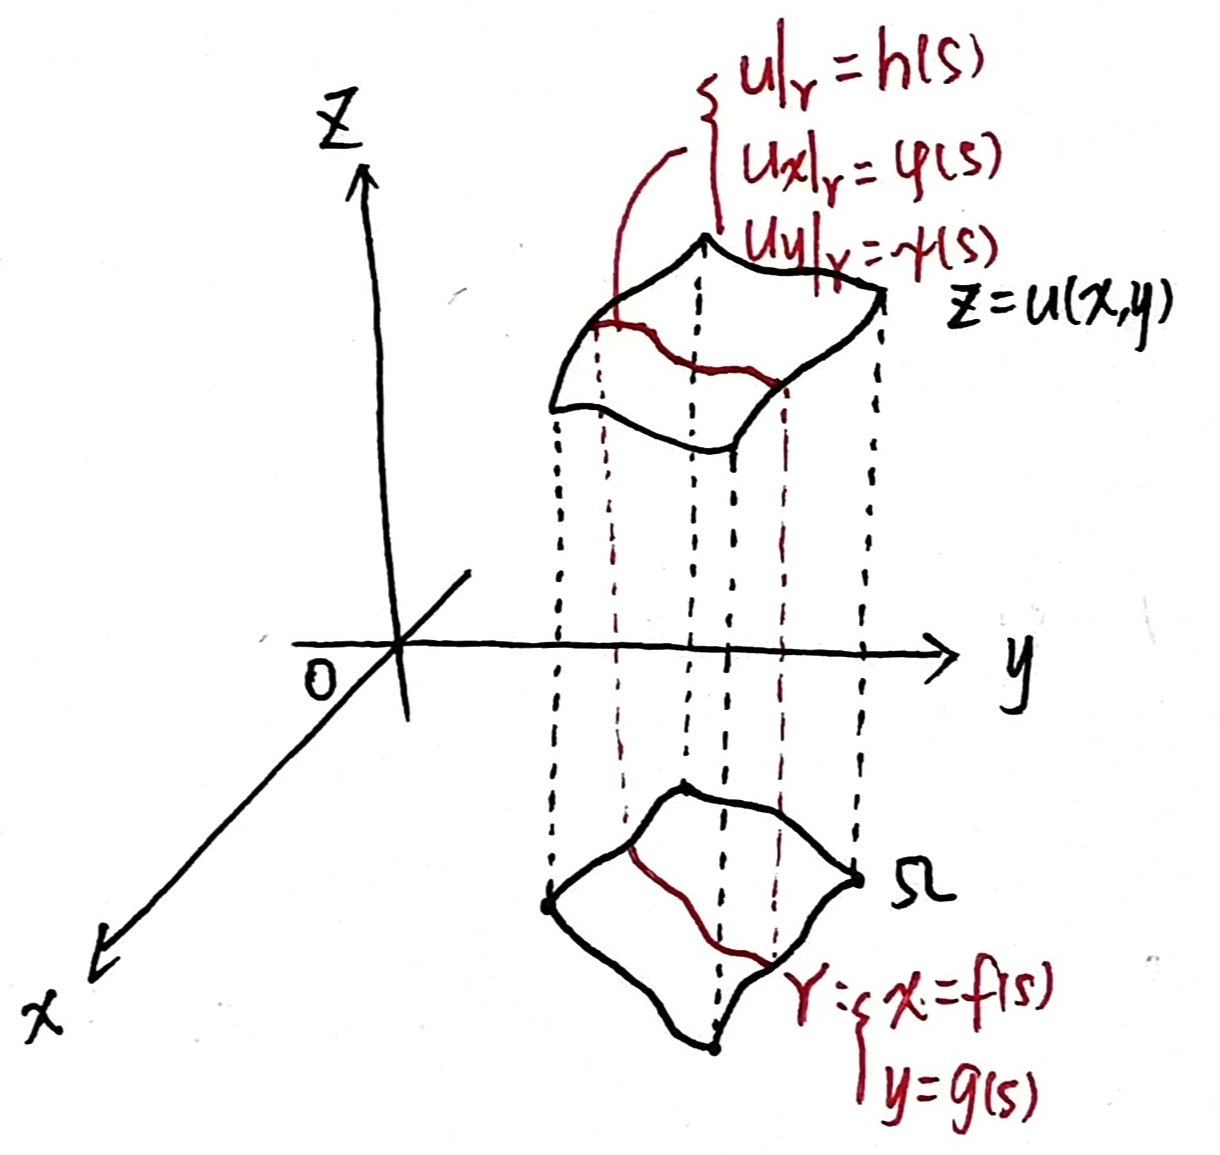
\includegraphics[width=0.45\linewidth]{figure/2.1-1}
		\caption{Cauchy Problelm for Quasi-Linear Second-Order Equation}
		\label{pic : 2.1-1} % 添加图像引用标签
	\end{figure}

	对(\ref{2.2}) 中Cauchy data等式左右两侧对$s$ 求导, 同时结合原方程(\ref{2.1}), 可得到在$\gamma$ 所对应的积分曲面区域上, 有关系式
	\begin{align*}
		\begin{cases}
			f^{'} u_{xx} + g^{'} u_{xy} = \varphi^{'} \\
			f^{'} u_{xy} + g^{'} u_{yy} = \psi^{'} \\
			au_{xx} + 2bu_{xy} + cu_{yy} = d
		\end{cases}
	\end{align*}
	i.e.
	\begin{align*}
		\begin{pmatrix}
			f^{'} &g^{'} &0 \\
			0 &f^{'} &g^{'} \\
			a &2b &c
		\end{pmatrix}
		\begin{pmatrix}
			u_{xx} \\
			u_{xy} \\
			u_{yy}
		\end{pmatrix} 
		= 
		\begin{pmatrix}
			\varphi^{'} \\
			\psi^{'} \\
			d
		\end{pmatrix}
	\end{align*}
	考虑系数矩阵行列式
	\begin{align*}
		\widetilde{\Delta} = 
		\begin{vmatrix}
			f^{'} &g^{'} &0 \\
			0 &f^{'} &g^{'} \\
			a &2b &c
		\end{vmatrix}
		= a(g^{'})^2 - 2b f^{'} g^{'} + c(f^{'})^2
	\end{align*}
	
	\vspace*{4em}
	
	\hspace*{-1.85em}Fix $P_0 = (f(s_0) , g(s_0) , h(s_0)) \in Graph(\varphi|_{\gamma})$, 
	
	\vspace*{2em}
	
	\hspace*{-1.85em}下面根据$\Delta$ 是否为零可给出该Cauchy问题解的存在性讨论:
	
	\newpage
	
	\begin{itemize}
		\item 若$\widetilde{\Delta}|_{P_0} \neq 0$, then \\
		By \textbf{Cramer's Rule}, $u_{xx} , u_{xy} , u_{yy}$ can be uniquely determined near $P_0$. \\
		而我们已知$\gamma$ 上$u$ 及一阶导数$u_x , u_y$ 解析式$\,\, \Rightarrow \,\,$ $u$ 的各阶导数可确定 ($u$ 足够光滑). \\
		If $u$ analytic, then u 在$P_0$ 附近的解析式可被唯一确定. 从而此时可得到$P_0$ 附近$u$ 的解. 
		
		\vspace*{2em}
		
		\item $\widetilde{\Delta}|_{P_0} = 0$ 
		\begin{align*}
			\Leftrightarrow \,\, a \Big( \frac{dy}{dt} \Big)^2 - 2b \Big( \frac{dy}{dt} \Big) \cdot \Big( \frac{dx}{dt} \Big) + c \Big( \frac{dx}{dt} \Big)^2 = 0 \,\, 
			&\Leftrightarrow \,\, a(dy)^2 - 2b(dx)(dy) + c(dx)^2 = 0 \\
			&\Leftrightarrow \,\, a \Big( \frac{dy}{dx} \Big)^2 - 2b \frac{dy}{dx} + c = 0 \\
			&\Leftrightarrow \,\, \frac{dy}{dx} = \frac{b \pm \sqrt{b^2 - ac}}{a}
		\end{align*}
		不难得到此时$P_0$ 在平面$xOy$ 上的投影落在满足方程$\dfrac{dy}{dx} = \dfrac{b \pm \sqrt{b^2 - ac}}{a}$ 的曲线上. 
	\end{itemize}
	
	\vspace*{4em}
	
	\hspace*{-1.85em}基于上述讨论, 我们给出\textbf{含2个自变量的2阶Quasi-Linear Equation}的\textbf{特征方程}、\textbf{特征线}等概念, 并给出\textbf{2阶Quasi-Linear Equation} 的分类. 
	
	\vspace*{3em}
	
	\begin{defn}\label{def 2.1.1}
		对于含2个自变量的2阶Quasi-Linear Equation, 
		\begin{align}
			au_{xx} + 2b u_{xy} + cu_{yy} = d \label{2.3}
		\end{align}
		where $a , b , c , d$ depend on $(x , y , u , u_x , u_y)$. 我们称方程
		\begin{align}
			a(dy)^2 - 2b(dx)(dy) + c(dx)^2 = 0 \label{2.4}
		\end{align}
		为该Quasi-Linear Equation的\underline{\textcolor{blue}{\textbf{特征方程}}}. 称$xOy$ 平面上满足方程
		\begin{align}
			\frac{dy}{dx} = \frac{b \pm \sqrt{b^2 - ac}}{a}
		\end{align}
		的曲线称为该Quasi-Linear Equation的\underline{\textcolor{blue}{\textbf{特征线}}}. 并对方程(\ref{2.3})给出如下分类: 
		
		\vspace*{1em}
		
		\begin{itemize}
			\item $\Delta = b^2 - ac < 0 \,\, \Rightarrow \,\,$ \underline{\textcolor{blue}{\textbf{elliptic (椭圆方程)}}}
			
			\item $\Delta = b^2 - ac > 0 \,\, \Rightarrow \,\,$ \underline{\textcolor{blue}{\textbf{hyperbolic (双曲方程)}}}
			
			\item $\Delta = b^2 - ac = 0 \,\, \Rightarrow \,\,$ \underline{\textcolor{blue}{\textbf{parabolic (抛物方程)}}}
		\end{itemize}
		
		\newpage
		
		\begin{rmk}
			\begin{itemize}
				\item 不难理解, 该分类为\textbf{局部概念}, 即在积分曲面$z = u(x , y)$ 的不同区域上, 方程的分类可能有所不同. 
				
				\vspace*{2em}
				
				\item 对于\textbf{Linear Equation}, 还可定义\textbf{特征曲面}、\textbf{特征方向}等\textbf{特征理论}, 详情可见书\footnote{参考书籍:\textbf{《数学物理方程讲义 (第二版)》--  姜礼尚、陈亚浙、刘西垣、易法槐} -- 第5章}. 
				
				\vspace*{2em}
				
				\item Fix $P_0 \in \gamma$. 对于\textbf{椭圆方程 (elliptic)}, 其在$P_0$ 附近不存在实特征线;对于\textbf{双曲方程 (hyperbolic)}, 其在$P_0$ 附近存在两族不同的实特征线;对于\textbf{抛物方程 (parabolic)}, 其在$P_0$ 点附近存在一族实特征线. 
				
				\vspace*{2em}
				
				\item 设$\varphi(x , y) = C$ 为一族特征线, 即满足特征方程(\ref{2.4}), i.e.
				\[ a \Big( \frac{dy}{dx} \Big)^2 - 2b \frac{dy}{dx} + c = 0 \]
				由于$\varphi(x , y) = C$, 因此$\varphi_{x} dx + \varphi_y dy = 0$, thus
				\[ 
				\frac{dy}{dx} = - \frac{\varphi_x}{\varphi_y} 
				\,\, \Rightarrow \,\, 
				a \Big( - \frac{\varphi_x}{\varphi_y} \Big)^2 + 2b \frac{\varphi_x}{\varphi_y} + c = 0 
				\]
				i.e.
				\[ a \varphi_{x}^2 + 2b \varphi_x \varphi_y + c \varphi_{y}^2 = 0 \]
			\end{itemize}
		\end{rmk}
	\end{defn}
	
	\vspace*{4em}
	
	根据前面的讨论, 对于方程(\ref{2.3})在曲线$\gamma$ 上一点$P_0$, 若$\widetilde{\Delta}|_{P_0} \neq 0$ 且$u$ 解析, 则$u$ 在$P_0$ 附近可由幂级数展开式唯一确定. 基于此, 对于\textbf{Hyperbolic Equation (双曲方程)}, 给出如下命题. 
	
	\vspace*{4em}
	
	\begin{proposition}\label{prop 2.1.1}
		\textbf{[Propagation of Singularity]}. 
		\begin{center}
			\textbf{对于Hyperbolic情形, 解本身或其导数的间断 (不连续)等奇异情况只会发生在特征线上}. 
		\end{center}
		
		\vspace*{2em}
		
		\begin{proof}
			在特征线外, $\Delta \neq 0$, $u_{xx} , u_{xy} , u_{yy}$ 可解. 
			\begin{center}
				(此处命题和证明都只给出了大致的叙述, 详细严谨的讨论可参见书籍\footnote{参考书籍:\textbf{《Partial Differential Equations》 -- Fritz John} -- $\S 2.2$ \textbf{Propagation of Singularities}. })
			\end{center}
		\end{proof}
	\end{proposition}

\newpage

\section{The Linear Second-Order Equation}
	这一节我们主要来对一般的\textbf{含2个自变量的2阶Linear Equation}进行化简分类, 即
	\begin{align}
		au_{xx} + 2bu_{xy} + cu_{yy}+  2du_{x} + 2eu_{y} + fu = 0 \label{2.6}
	\end{align}
	where coefficients $a , b , c , d , e , f$ depend on $(x , y)$.  
	
\vspace*{2em}
	
\subsection{含2个自变量的2阶Linear Equation的标准型}
	
	\vspace*{2em}
	
	首先先来给出\textbf{标准型}的概念. 
	
	\vspace*{1em}
	
	\begin{defn}\label{def 2.2.1}
		对于如下3种形式的方程
		\begin{align}
			\begin{cases}
				\dfrac{\partial^2 u}{\partial t^2} - a^2 \Delta u = f \hspace*{2em} &\text{(波动方程)} \\
				\dfrac{\partial u}{\partial t} - a^2 \Delta u = f &\text{(热传导方程)} \\
				- \Delta u = f &\text{(位势方程)}
			\end{cases}
		\end{align}
		上述三个方程分别称为\underline{\textcolor{blue}{\textbf{双曲型 (Hyperbolic)}}}、\underline{\textcolor{blue}{\textbf{抛物型 (Parabolic)}}}和\underline{\textcolor{blue}{\textbf{椭圆型 (Elliptic)的标准型}}}. 
		
		\vspace*{2em}
		
		\begin{rmk}
			对\textbf{含2个自变量的2阶Linear Equation}进行化简分类的工作, 即将方程(\ref{2.6}) 经过变量代换后 (线性 / 非线性), 其\textbf{二阶项}被化为标准型. 而对于\textbf{含2个自变量}的情形, 上述标准型可简化表达为
			\begin{align*}
				\begin{cases}
					u_{tt} - a^2 u_{xx} = f \\
					u_{t} - a^2 u_{xx} = f \\
					- u_{xx} = f
				\end{cases}
			\end{align*}
		\end{rmk}
	\end{defn}

\newpage

\subsection{含2个自变量的2阶Linear Equation的化简}
	Suppose $\Omega \subset xOy$ 为积分曲面$z = u(x , y)$ 在平面$xOy$ 上的投影区域. Fix $P_0 = (x_0 , y_0) \in \Omega$. 下面对方程(\ref{2.6}) 在$P_0$ 点附近的区域化简为\textbf{标准型 (Def \ref{def 2.2.1})}. 
	
	\vspace*{2em}
	
	\hspace*{-1.85em}下面针对方程(\ref{2.6}) 在点$P_0$ 附近的类型, 分为3种情况进行讨论:
	
	\vspace*{1em}
	
	\begin{enumerate}
		\item \textbf{\underline{Hyperbolic ($\Delta = b^2 - ac > 0$, 双曲方程)}}:
		
		\vspace*{1em}
		
		根据$\S 2.1$ 节的讨论 (\textbf{Def \ref{def 2.1.1}}), 通过求解特征方程
		\begin{align*}
			\frac{dy}{dx} = \frac{b \pm \sqrt{b^2 - ac}}{a}
		\end{align*}
		可得到两族实特征线$\varphi(x , y) = C$ 与$\psi(x , y) = C$. 令
		\begin{align}
			\xi = \varphi(x , y) , \,\, \eta = \psi(x , y) \label{2.8}
		\end{align}
		不难证明上述变换可逆\footnote{由于$\varphi(x , y) = C$, 因此$\varphi_x dx + \varphi_y dy = 0 \,\, \Rightarrow \,\, \dfrac{dy}{dx} = -\dfrac{\varphi_x}{\varphi_y}$. 因为$\varphi$ 满足特征方程(\ref{2.4}), 所以$-\dfrac{\varphi_x}{\varphi_y}$ 为方程$a \lambda^2 - 2b \lambda + c = 0$ 的解. 同理可说明$-\dfrac{\psi_x}{\psi_y}$ 为该方程两个不同的实根, 从而$-\dfrac{\varphi_x}{\varphi_y} \neq -\dfrac{\psi_x}{\psi_y} \,\, \Rightarrow \,\, J \neq 0$.}, 即
		\[ 
		J = \frac{\partial(\xi , \eta)}{\partial (x , y)} = 
		\begin{vmatrix}
			\varphi_x &\varphi_y \\
			\psi_x &\psi_y
		\end{vmatrix} \neq 0 
		\]
		经计算, 
		\begin{align*}
			\begin{cases}
				u_x = u_{\xi} \cdot \dfrac{\partial \varphi}{\partial x} + u_{\eta} \cdot \dfrac{\partial \psi}{\partial x} \\
				u_y = u_{\xi} \cdot \dfrac{\partial \varphi}{\partial y} + u_{\eta} \cdot \dfrac{\partial \psi}{\partial y}
			\end{cases} , \,\, 
			\begin{cases}
				u_{xx} = \cdots \\
				u_{xy} = \cdots \\
				u_{yy} = \cdots
			\end{cases}
		\end{align*}
		代入原方程(\ref{2.6}), 得到
		\begin{align}
			Au_{\xi\xi} + 2Bu_{\xi\eta} + Cu_{\eta\eta} + \cdots = 0 \label{2.9}
		\end{align}
		where 
		\begin{align*}
			\begin{cases}
				A = a \varphi_{x}^2 + 2b \varphi_x \varphi_y + c\varphi_{y}^2 \\
				B = a \varphi_x \psi_x + b \Big( \varphi_x \psi_y + \varphi_y \psi_x \Big) + c \varphi_y \psi_y \\
				C = a \psi_{x}^2 + 2b \psi_x \psi_y + c\psi_{y}^2
			\end{cases}
		\end{align*}
		
		\newpage
		
		Since $\varphi(x , y) = C$ and $\psi(x , y) = C$ 为方程(\ref{2.6}) 的两族特征线, then by \textbf{特征线方程所满足的关系 (Def \ref{def 2.1.1})}, 
		\begin{align*}
			a \varphi_{x}^2 + 2b \varphi_x \varphi_y + c\varphi_{y}^2 = 0 \,\,\,\, \text{and} \,\,\,\, a \psi_{x}^2 + 2b \psi_x \psi_y + c\psi_{y}^2 = 0
		\end{align*}
		i.e. $A = C = 0$. 可以计算证明$B \neq 0$, 等式(\ref{2.9})两侧除去$2B$, 得到
		\[ u_{\xi\eta} + 2D u_{\xi} + 2E u_{\eta} + Fu = 0 \]
		为了消去交叉项$u_{\xi\eta}$, 此时再进行一次变量代换
		\[ x^{'} = \xi + \eta , \,\, y^{'} = \xi - \eta \]
		可将方程化简为
		\[ u_{y^{'}y^{'}} - u_{x^{'}x^{'}} + 2D^{'} u_{x^{'}} + 2E^{'}u_{y^{'}} + F^{'}u = 0 \]
		此即得到了二次项化简为\textbf{双曲标准型 (Def \ref{def 2.2.1})}的结果. 
		
		\newpage
		
		\item \textbf{\underline{Parabolic ($\Delta = b^2 - ac = 0$, 抛物方程)}}:
		
		\vspace*{1em}
		
		由于$\Delta = b^2 - ac = 0$, 因此求解特征方程可得到一族特征曲线$\varphi(x , y) = C$. 此时任取函数$\psi(x , y) = C$, $\st \varphi$ 与$\psi$ 线性无关, 令
		\[ \xi = \varphi(x , y) , \,\, \eta = \psi(x , y) \]
		同理, 可通过计算得到
		\[ Au_{\xi\xi} + 2Bu_{\xi\eta} + Cu_{\eta\eta} + \cdots = 0 \]
		where 
		\begin{align*}
			\begin{cases}
				A = a \varphi_{x}^2 + 2b \varphi_x \varphi_y + c\varphi_{y}^2 \\
				B = a \varphi_x \psi_x + b \Big( \varphi_x \psi_y + \varphi_y \psi_x \Big) + c \varphi_y \psi_y \\
				C = a \psi_{x}^2 + 2b \psi_x \psi_y + c\psi_{y}^2
			\end{cases}
		\end{align*}
		Similarly, since $\varphi(x , y) = C$ 为特征线, then by \textbf{特征线方程所满足的关系 (Def \ref{def 2.1.1})}, 
		\[ a \varphi_{x}^2 + 2b \varphi_x \varphi_y + c\varphi_{y}^2 = 0 \]
		Thus $A = 0$. \\
		Since $\Delta = b^2 - ac = 0$, then $b = \pm\sqrt{ac}$. 不妨设$a , b , c \geq 0$, then
		\begin{align*}
			B 
			&= a \varphi_x \psi_x + b \Big( \varphi_x \psi_y + \varphi_y \psi_x \Big) + c \varphi_y \psi_y \\
			&= \Big( \sqrt{a} \varphi_x + \sqrt{c} \varphi_y \Big) \Big( \sqrt{a} \psi_x + \sqrt{c} \psi_y \Big)
		\end{align*}
		Since $a \varphi_{x}^2 + 2b \varphi_x \varphi_y + c\varphi_{y}^2 = 0$, $b = \sqrt{ac}$, then
		\[ a \varphi_{x}^2 + 2b \varphi_x \varphi_y + c\varphi_{y}^2 = \Big( \sqrt{a} \varphi_x + \sqrt{c} \varphi_y \Big)^2 = 0 \]
		Hence $A = B = 0$. 方程可化为
		\[ u_{\eta\eta} + 2D u_{\xi} + 2E u_{\eta} + Fu = 0 \]
		对比\textbf{抛物方程的标准型 (Def \ref{def 2.2.1})}, 为了消去$u_{\eta}$, 再令
		\begin{align*}
			v = u e^{\tfrac{1}{2} \int_{\eta_0}^{\eta} 2E(\xi , \tau) \, d\tau}
		\end{align*}
		从而可得到二次项化为\textbf{抛物方程的标准型 (Def \ref{def 2.2.1})}的结果
		\[ v_{\eta\eta} + 2D^{'} v_{\xi} + F^{'}v = 0 \]
		
		\newpage
		
		\item \textbf{\underline{Elliptic ($\Delta = b^2 - ac < 0$, 椭圆方程)}}:
		
		\vspace*{1em}
		
		对于实数域$\R$ 上的情形\footnote{若放宽至复数域$\C$ 上进行化简, 则过程将是Trivial的, 详情可见书籍:\textbf{《数学物理方程讲义 (第二版)》--  姜礼尚、陈亚浙、刘西垣、易法槐} -- 第五章$\S$2 第253页.}, 我们先引入变量替换, 而后再给出所需条件求解该替换方程, i.e.
		\[ \xi = \varphi(x , y) , \,\, \eta = \psi(x , y) \]
		同理可得到
		\[ Au_{\xi\xi} + 2Bu_{\xi\eta} + Cu_{\eta\eta} + \cdots = 0 \]
		where 
		\begin{align*}
			\begin{cases}
				A = a \varphi_{x}^2 + 2b \varphi_x \varphi_y + c\varphi_{y}^2 \\
				B = a \varphi_x \psi_x + b \Big( \varphi_x \psi_y + \varphi_y \psi_x \Big) + c \varphi_y \psi_y \\
				C = a \psi_{x}^2 + 2b \psi_x \psi_y + c\psi_{y}^2
			\end{cases}
		\end{align*}
		参考\textbf{椭圆方程的标准型 (Def \ref{def 2.2.1})}, 我们要化简的目标形式应为
		\[ u_{\xi\xi} + u_{\eta\eta} + 2Du_{\xi} + 2Eu_{\eta} + Fu = 0 \]
		可以验证的是, 当$\varphi$ 与$\psi$ 满足下述条件时, 
		\begin{align*}
			\begin{cases}
				\varphi_x = \dfrac{b\psi_x + c\psi_y}{W} \\
				\varphi_y = - \dfrac{a\psi_x + b\psi_y}{W}
			\end{cases} , \,\, W = \sqrt{ac - b^2}
		\end{align*}
		此时可得到$A = C$, $B = 0$. 从而即可得到目标形式. \\
		而上述条件所需的必要条件为求解下述方程 (\textbf{Beltrami Equation})
		\begin{align*}
			\Big( \frac{b \psi_x + c\psi_y}{W} \Big)_y + \Big( \frac{a\psi_x + b\psi_y}{W} \Big)_x = 0
		\end{align*}
	\end{enumerate}
	
	\newpage
	
	下面给出一个例子. 
	
	\begin{example}\label{ex 2.2.1}
		\textbf{[The Tricomi Equation]}. 
		\begin{center}
			$u_{yy} - y u_{xx} = 0$
		\end{center}
		
		\vspace*{2em}
		
		\begin{solution}
			在一般形式下
			\[ au_{xx} + 2b u_{xy} + c u_{yy} = d \]
			$a = -y , \,\, b = 0 , \,\, c = 1$. 计算得到$\Delta = b^2 - ac = y$. 于是方程可分类为:
			\begin{align*}
				\begin{cases}
					y > 0 , \,\, \text{Hyperbolic (双曲方程)} \\
					y = 0 , \,\, \text{Parabolilc (抛物方程)} \\
					y < 0 , \,\, \text{Elliptic (椭圆方程)}
				\end{cases}
			\end{align*}
			For $y > 0$, calculate the characteristic equation
			\[ \frac{dy}{dx} = \frac{b \pm \sqrt{b^2 - ac}}{a} = \pm \frac{1}{\sqrt{y}} \]
			i.e. 特征曲线为
			\[ 3x \pm 2y^{\tfrac{3}{2}} = C \]
			Let 
			\[ \xi = 3x - 2y^{\tfrac{3}{2}} , \,\, \eta = 3x + 2y^{\tfrac{3}{2}} \]
			得到
			\[ u_{\xi\eta} - \frac{1}{6} \frac{u_{\xi} - u_{\eta}}{\xi - \eta} = 0 \]
			为了消去交叉项$u_{\xi\eta}$, let
			\[ x^{'} = \xi + \eta , \,\, y^{'} = \xi - \eta \]
			Then
			\begin{align*}
				u_{\xi} = u_{x^{'}} \frac{\partial x^{'}}{\partial \xi} + u_{y^{'}} \frac{\partial y^{'}}{\partial \xi} = u_{x^{'}} + u_{y^{'}} 
				\hspace*{1em} , \hspace*{1em}
				u_{\eta} = u_{x^{'}} \frac{\partial x^{'}}{\partial \eta} + u_{y^{'}} \frac{\partial y^{'}}{\partial \eta} = u_{x^{'}} - u_{y^{'}}
			\end{align*}
			And
			\begin{align*}
				u_{\xi\eta} 
				= \Big( u_{\xi} \Big)_{\eta} 
				= \Big( u_{\xi} \Big)_{x^{'}} \frac{\partial x^{'}}{\partial \eta} + \Big( u_{\xi} \Big)_{y^{'}} \frac{\partial y^{'}}{\partial \eta} 
				&= \Big( u_{\xi} \Big)_{x^{'}} - \Big( u_{\xi} \Big)_{y^{'}} \\
				&= \Big( u_{x^{'}x^{'}} + u_{x^{'}y^{'}} \Big) - \Big( u_{x^{'}y^{'}} + u_{y^{'}y^{'}} \Big) 
				= u_{x^{'}x^{'}} - u_{y^{'}y^{'}}
			\end{align*}
			代入可解得
			\begin{align*}
				u_{x^{'}x^{'}} - u_{y^{'}y^{'}} + \frac{1}{3y^{'}} u_{y^{'}} = 0 , \,\, \text{when} \,\,  y > 0
			\end{align*}
		\end{solution}
	\end{example}

\newpage

\section{The One-Dimensional Wave Equation}
	这一节我们将在两种不同的边界条件上, 给出\textbf{一维波动方程}的两种不同解法 (\textbf{特征线法}和\textbf{分离变量法}), 并将给出其\textbf{解的存在唯一性}讨论. 
	
\subsection{一维齐次波动方程的特征线法 (上半空间, D'Alembert, 能量不等式)}
	对于在\underline{\textbf{上半空间}$\R \times [0 , \infty)$} 上考虑一般的一维波动方程的初值问题:
	\begin{align}
		\begin{cases}
			\dfrac{\partial^2 u}{\partial t^2} - c^2 \dfrac{\partial^2 u}{\partial x^2} = f(x , t) , \,\, x \in \R , t > 0 \\
			u \Big|_{t = 0} = \varphi(x) \\
			u_t \Big|_{t = 0} = \psi(x)
		\end{cases}\label{2.10}
	\end{align}

	\vspace*{1em}
	
	根据\textbf{线性PDE的叠加原理 (Thm \ref{thm A.2.1})}, 该方程的解可写为如下两个子问题的解的和:
	
	\begin{align*}
		\begin{cases}
			\dfrac{\partial^2 u}{\partial t^2} - c^2 \dfrac{\partial^2 u}{\partial x^2} = 0 , \,\, x \in \R , t > 0 \\
			u \Big|_{t = 0} = \varphi(x) \\
			u_t \Big|_{t = 0} = \psi(x)
		\end{cases} , \,\,\,\, 
		\begin{cases}
			\dfrac{\partial^2 u}{\partial t^2} - c^2 \dfrac{\partial^2 u}{\partial x^2} = f(x , t) , \,\, x \in \R , t > 0 \\
			u \Big|_{t = 0} = 0 \\
			u_t \Big|_{t = 0} = 0
		\end{cases}
	\end{align*}
	
	\vspace*{2em}
	
	又根据\textbf{一维波动方程的齐次性原理 (Thm \ref{thm A.3.1})}, 事实上只需求解第一个\textbf{齐次初值问题}的解, 在后面我们也将给出有关\textbf{解的存在唯一性}的严谨讨论. 
	
	\vspace*{6em}
	
	对于一维齐次波动方程
	\begin{align}
		\begin{cases}
			\dfrac{\partial^2 u}{\partial t^2} - c^2 \dfrac{\partial^2 u}{\partial x^2} = 0 , \,\, x \in \R , t > 0 \\
			u \Big|_{t = 0} = \varphi(x) \\
			u_t \Big|_{t = 0} = \psi(x)
		\end{cases}\label{2.11}
	\end{align}
	解的存在唯一性问题, 下面给出定理. 
	
	\newpage
	
	\begin{thm}\label{thm 2.3.1}
		\textbf{[一维齐次波动方程, D'Alembert, 能量不等式]}. \\
		If $\varphi \in C^2(\R)$, $\psi \in C^1(\R)$, then for the problem (\ref{2.11})
		\begin{align*}
			\begin{cases}
				\dfrac{\partial^2 u}{\partial t^2} - c^2 \dfrac{\partial^2 u}{\partial x^2} = 0 , \,\, x \in \R , t > 0 \\
				u \Big|_{t = 0} = \varphi(x) \\
				u_t \Big|_{t = 0} = \psi(x)
			\end{cases}
		\end{align*}
		It has a unique solution $u \in C^2 \Big( \R \times (0 , \infty) \Big) \cap C^1 \Big( \R \times [0 , \infty) \Big)$:
		\begin{align}
			u(x , t) = \frac{1}{2} \Big[ \varphi(x + ct) + \varphi(x - ct) \Big] + \frac{1}{2c} \int_{x - ct}^{x + ct} \psi(\xi) \, d\xi \label{2.12}
		\end{align}
		which is called the \underline{\textcolor{blue}{\textbf{D'Alembert Formula}}}. 
		
		\vspace*{8em}
		
		\begin{rmk}
			$\forall$ fixed $(x_0 , t_0) \in \R \times (0 , \infty)$, by \textbf{D'Alembert Formula}, 解$u(x , t)$ 在该点处取值
			\[ u(x_0 , t_0) = \frac{1}{2} \Big[ \varphi(x_0 + ct_0) + \varphi(x_0 - ct_0) \Big] + \frac{1}{2c} \int_{x_0 - ct_0}^{x_0 + ct_0} \psi(\xi) \, d\xi \]
			故$u$ 在点$(x_0 , t_0)$ 处取值只与$\varphi$ 在$x_0 - ct_0 , x_0 + ct_0$ 两点处的取值, 以及$\psi$ 在区间$[x_0 - ct_0 , x_0 + ct_0]$ 上的取值有关. 基于此, 下面我们给出\textbf{依赖区间}、\textbf{决定区域}、\textbf{影响区域}等概念. 
			
			\begin{figure}[thbp!]
				\centering
				\begin{minipage}[t]{0.49\linewidth}
					\centering
					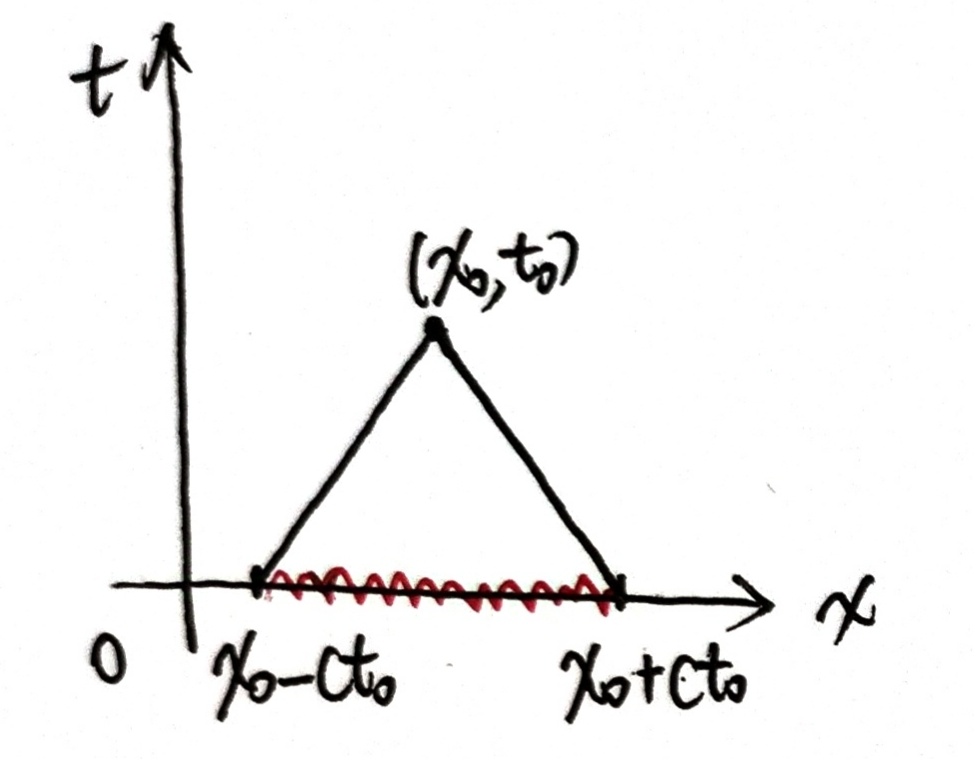
\includegraphics[width=0.5\linewidth]{figure/2.3-1}
					\caption{点$(x_0 , t_0)$ 的依赖区间}
					\label{fig : 2.3-1}
				\end{minipage}
				\begin{minipage}[t]{0.49\linewidth}
					\centering
					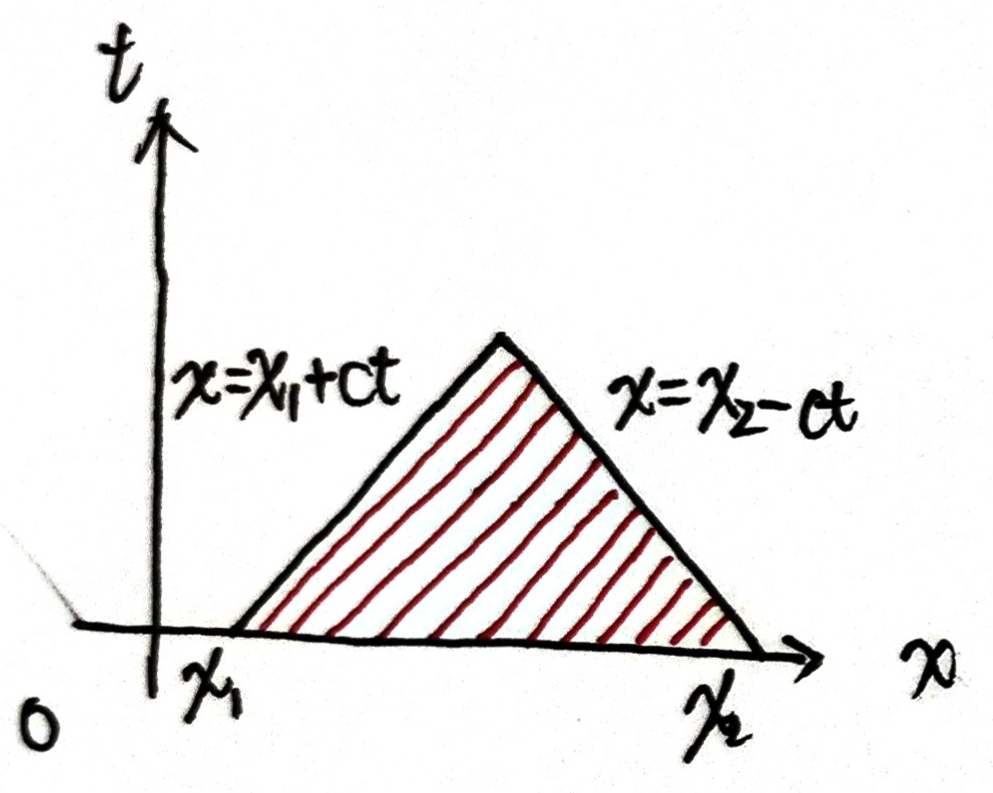
\includegraphics[width=0.5\linewidth]{figure/2.3-2}
					\caption{区间$[x_1 , x_2]$ 的决定区域}
					\label{fig : 2.3-2}
				\end{minipage}
			\end{figure}
		
			\vspace*{2em}
			
			\begin{defn}\label{def 2.3.1}
				\textbf{[依赖区间, 决定区域, 影响区域]\footnote{详细论述可参考:\textbf{《数学物理方程讲义 (第二版)》--  姜礼尚、陈亚浙、刘西垣、易法槐} -- $\S 2.2.3$ 依赖区间、决定区域和影响区域. }}. \\
				对于初值问题 (\ref{2.11}), 称$x$ 轴上的区间$[x_0 - ct_0 , x_0 + ct_0]$ 为点$(x_0 , t_0)$ 的\underline{\textcolor{blue}{\textbf{依赖区间}}}, 表示解$u(x , t)$ 在点$(x_0 , t_0)$ 处取值只与$\varphi$ 在$x_0 - ct_0 , x_0 + ct_0$ 两点处的取值, 以及$\psi$ 在区间$[x_0 - ct_0 , x_0 + ct_0]$ 上的取值有关, 而与其他点上的初始条件无关. 
				
				\newpage
				
				\hspace*{-1.85em}对于$x$ 轴上任一区间$[x_1 , x_2]$, 直线$x = x_1 + ct$ 与$x = x_2 - ct$ 一起围成一个三角形区域, 解$u(x , t)$ 在此三角形区域中任一点$(x_0 , t_0)$ 的依赖区间都完全落在$[x_1 , x_2]$ 中, 而与此区间外的初始条件无关, 这个区域称为区间$[x_1 , x_2]$ 的\underline{\textcolor{blue}{\textbf{决定区域}}}. 
				
				\vspace*{4em}
				
				\begin{figure}[thbp!]
					\centering
					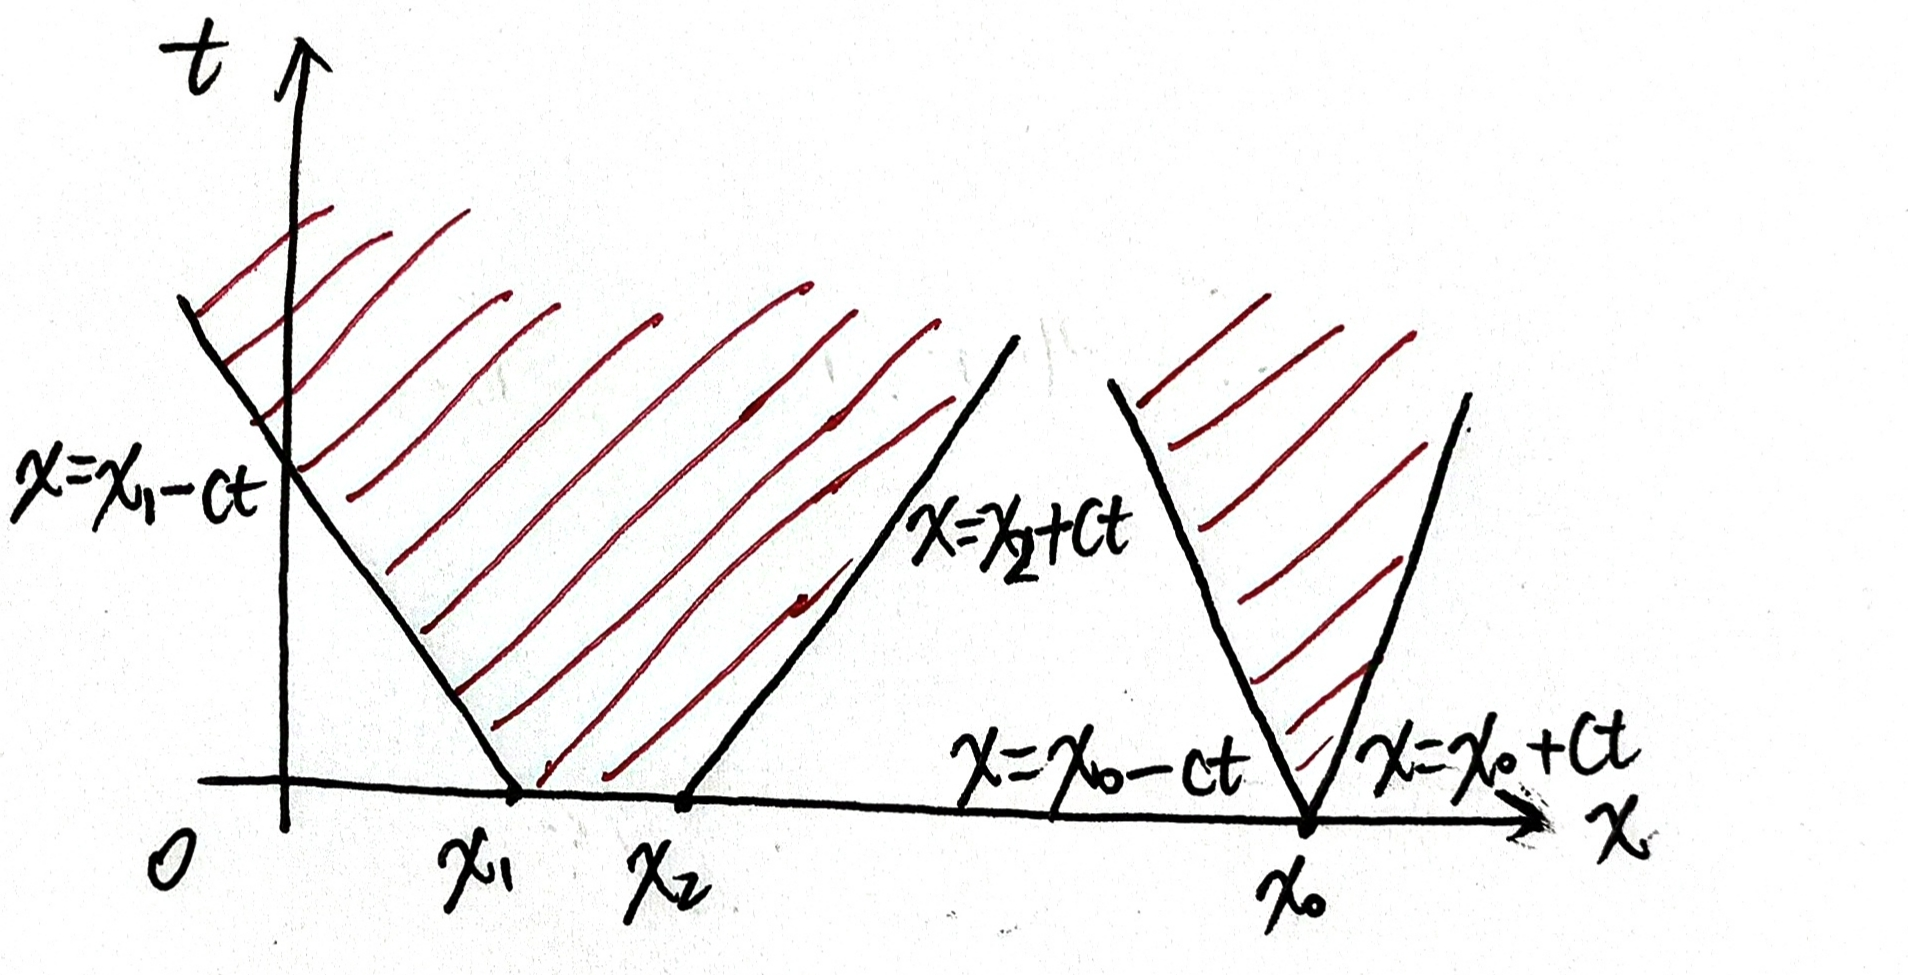
\includegraphics[width=0.5\linewidth]{figure/2.3-3}
					\caption{区间$[x_1 , x_2]$ 及点$x_0$ 的影响区域}
					\label{pic : 2.3-3} % 添加图像引用标签
				\end{figure}
			
				\vspace*{4em}
				
				\hspace*{-1.85em}对于$x$ 轴上任一区间$[x_1 , x_2]$, 区域
				\[ E = \Big\{ (x , t) \,\, \Big| \,\, x_1 - ct \leq x \leq x_2 + ct , \,\, t > 0 \Big\} \]
				中每一点的依赖区间都与$[x_1 , x_2]$ 有交集, 即解$u(x , t)$ 在其中任一点的取值都要受到区间$[x_1 , x_2]$ 上某些点处初始条件的影响, 称平面区域$E$ 为区间$[x_1 , x_2]$ 的\underline{\textcolor{blue}{\textbf{影响区域}}}. 特别地, 当$x_1 = x_2 = x_0$ 时, 我们可以得到一个点$x_0$ 的影响区域, 即定义域中函数值能被$x_0$ 处初始条件影响的范围. 
				
				
			\end{defn}
		\end{rmk}
		
		\vspace*{10em}
		
		\begin{proof}
			\begin{itemize}
				\item \textbf{存在性}:
				\begin{center}
					\textbf{[思路:先证明若有解, 则解满足上述形式;再将上述$u$ 回代至原问题, 证明它是解]}. 
				\end{center}
				\newpage
				假设原问题有解. 对于Hyperbolic Equation
				\[ u_{tt} - c^2 u_{xx} = 0 \]
				其特征方程为
				\[ (dx)^2 - c^2(dt)^2 = 0 \]
				得到两族实特征线$x \pm ct = C$. 下面进行可逆坐标变换 (合理性可见 (\ref{2.8})), 令
				\[ \xi = x + ct , \,\, \eta = x - ct \]
				经过计算, 原波动方程等价于
				\[ u_{\xi \eta} = 0 \]
				由此可知$u$ 中不含$\xi$ 与$\eta$ 的交叉项, 即可表示为
				\[ u(\xi , \eta) = F(\xi) + G(\eta) \]
				i.e. 
				\[ u(x , t) = F(x + ct) + G(x - ct) , \,\, x \in \R , t > 0 \]
				对于原初值问题 (\ref{2.11})的边界条件, 可转化为
				\begin{align*}
					\begin{cases}
						F(x) + G(x) = \varphi(x) \\
						cF^{'}(x) - c G^{'}(x) = \psi(x)
					\end{cases}
				\end{align*}
				Since $\varphi \in C^{2}(\R)$, then 
				\[ F^{'}(x) = \frac{1}{2c} \Big( c \varphi(x) + \psi(x) \Big) , \,\, G^{'}(x) = \frac{1}{2c} \Big( c \varphi(x) - \psi(x) \Big) \]
				对$x$ 积分, 结合$F(x) + G(x) = \varphi(x)$, 可得
				\begin{align*}
					\begin{cases}
						F(x) = \dfrac{1}{2c} \Big( c \varphi(x) + \int_{x_0}^x \psi(s) \, ds \Big) + \alpha \\
						G(x) = \dfrac{1}{2c} \Big( c \varphi(x) - \int_{x_0}^x \psi(s) \, ds \Big) + \beta \\
						\alpha + \beta = 0
					\end{cases}
				\end{align*}
				从而若原问题有解, 则解$u$ 可表达为
				\begin{align*}
					u(x , t) 
					&= F(x + ct) + G(x - ct) \\
					&= \frac{1}{2c} \Big[ c \varphi(x + ct) + \int_{x_0}^{x + ct} \psi(s) \, ds \Big] + \frac{1}{2c} \Big[ c \varphi(x - ct) - \int_{x_0}^{x - ct} \psi(s) \, ds \Big] \\
					&= \frac{1}{2} \Big[ \varphi(x + ct) + \varphi(x - ct) \Big] + \frac{1}{2c} \int_{x - ct}^{x + ct} \psi(s) \, ds
				\end{align*}
				将上述函数$u(x , t)$ 回代至原问题 (\ref{2.11}), 不难证明其就是原问题的一个解. 
				
				\newpage
				
				\item \textbf{唯一性}:\textbf{[利用 \underline{\textcolor{blue}{能量不等式}}进行证明]}. \\
				$\forall$ fixed $(x_0 , t_0) \in \R \times (0 , \infty)$, 根据\textbf{Def \ref{def 2.3.1}}, 我们可得到其依赖区间为$[x_0 - ct_0 , x_0 + ct_0]$ 及该区间的决定区域. 对于$\forall \tau \in [0 , t_0]$, 定义区域$K_\tau$ 如下
				
				\begin{figure}[thbp!]
					\centering
					\begin{minipage}[t]{0.59\linewidth}
						\centering
						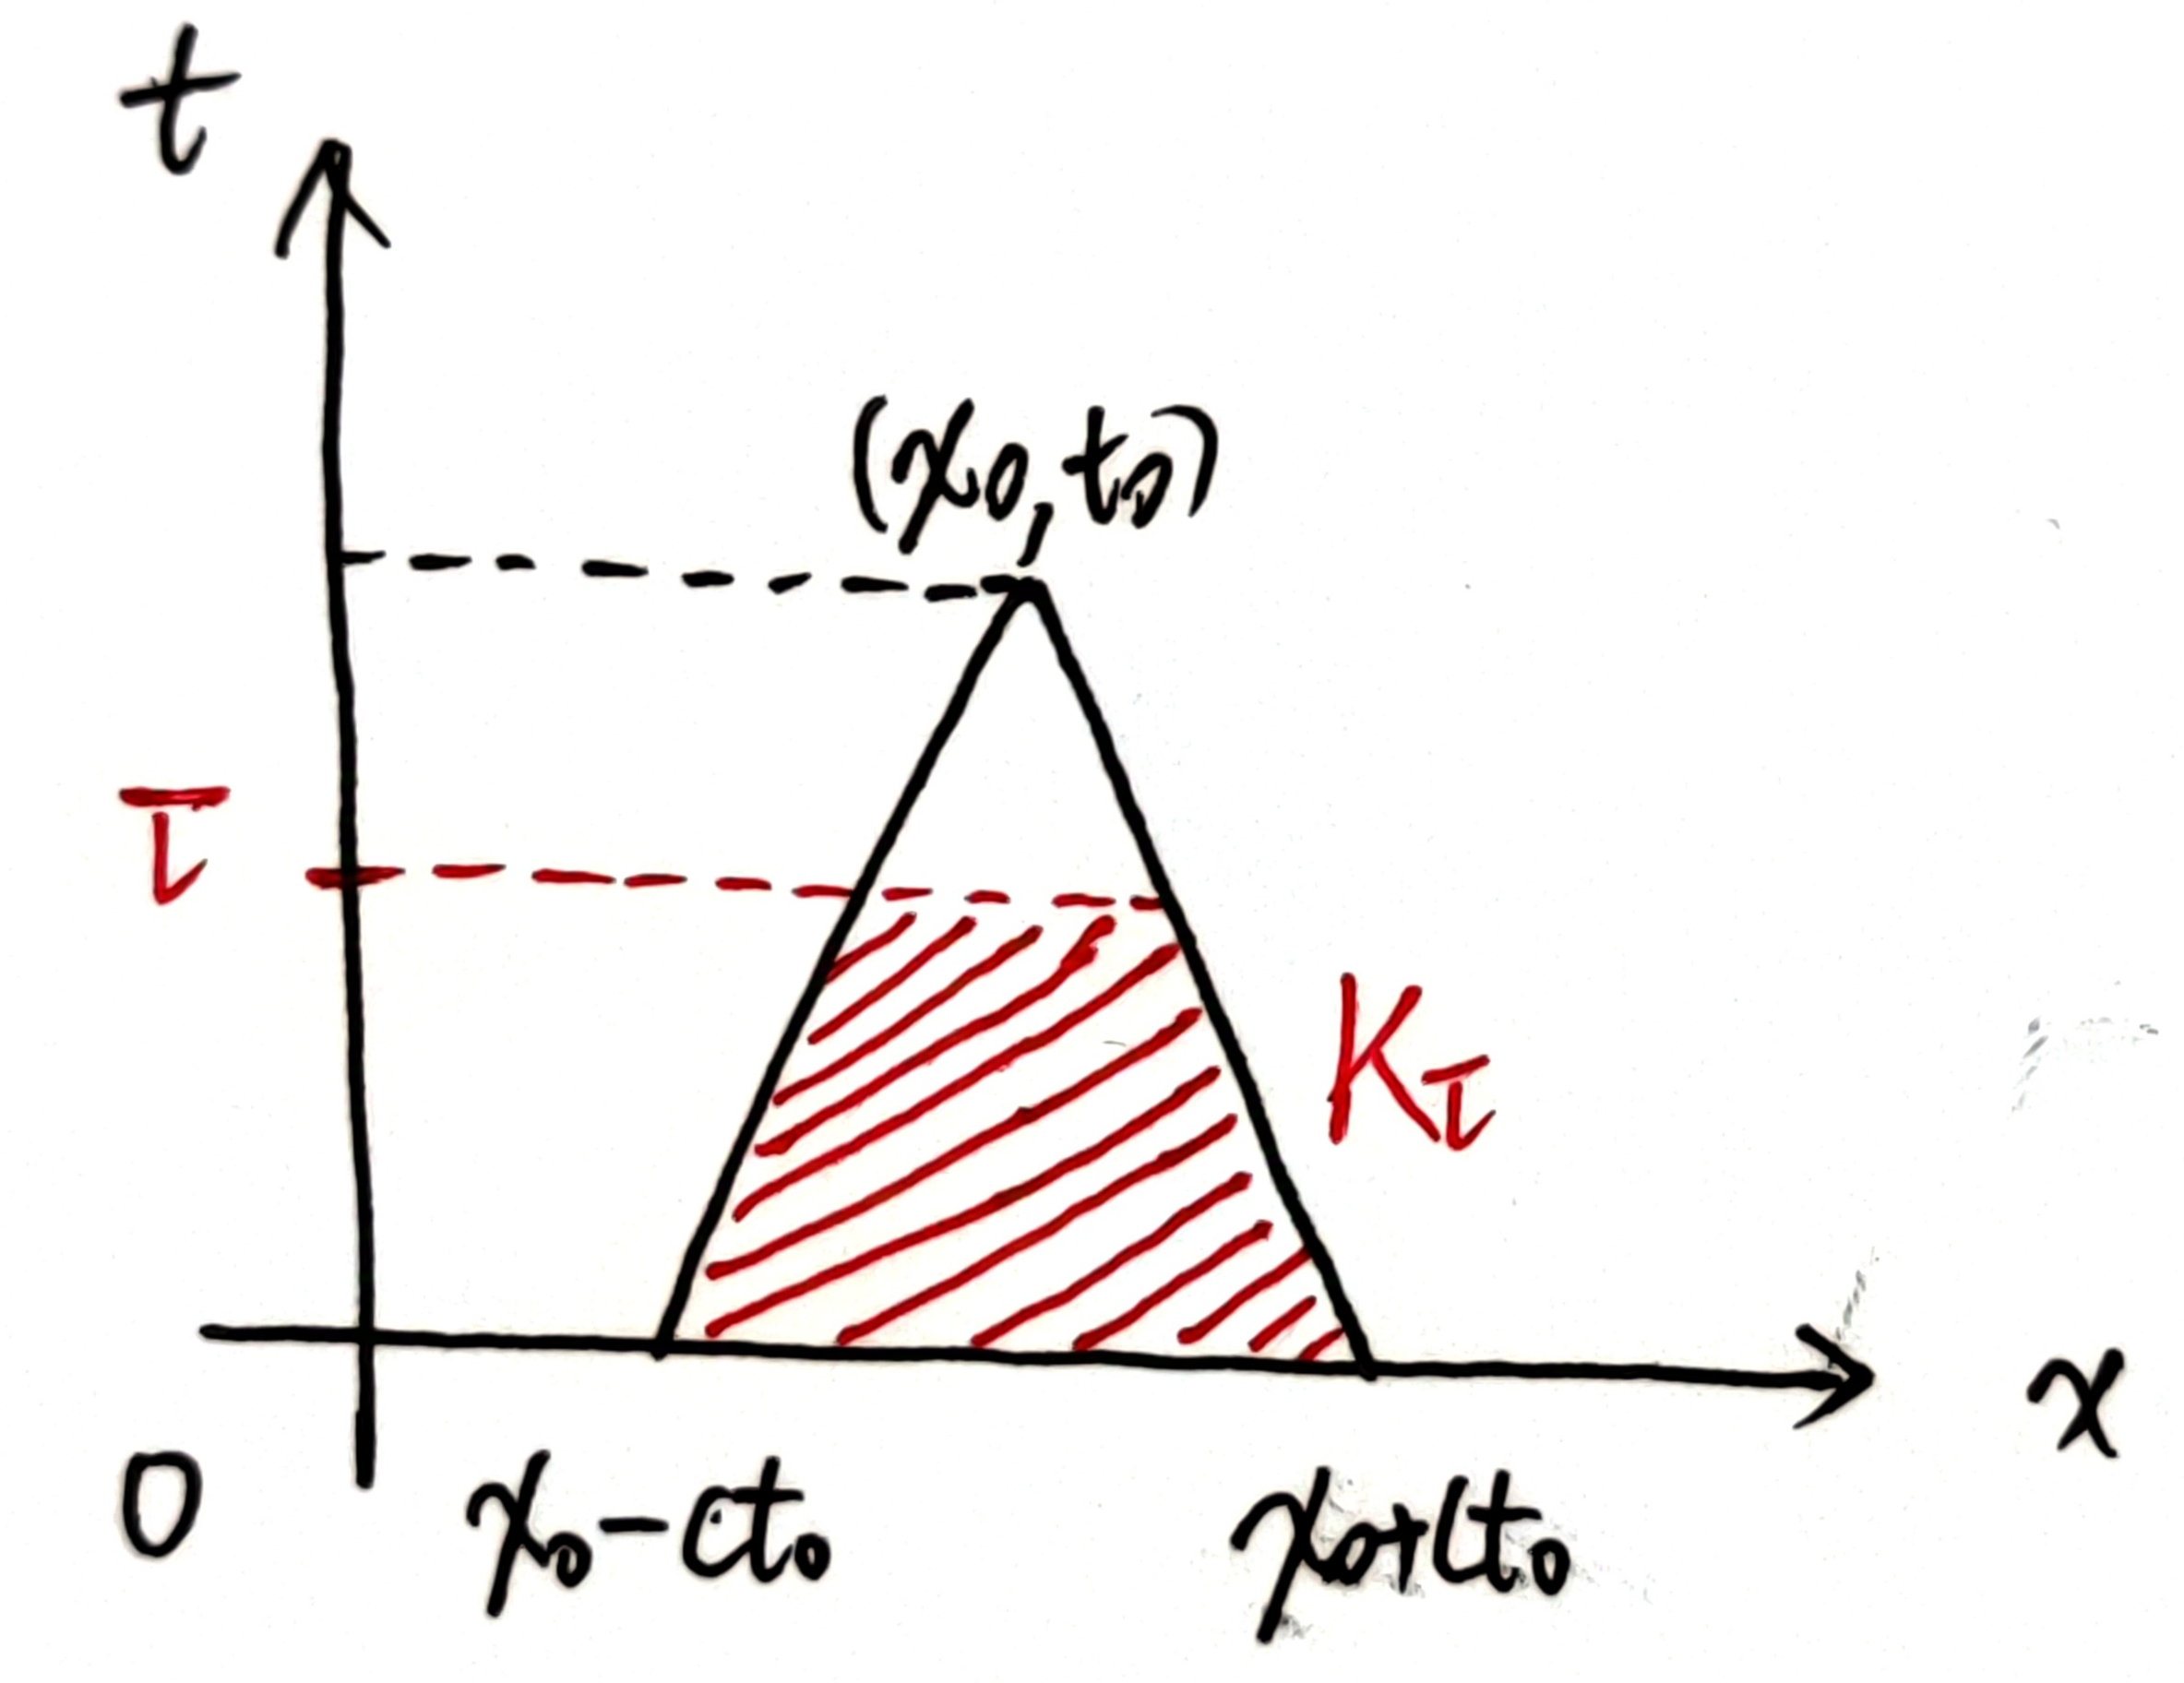
\includegraphics[width=0.6\linewidth]{figure/2.3-4}
						\caption{依赖区间及区域$K_\tau$ 的定义}
						\label{fig : 2.3-4}
					\end{minipage}
					\begin{minipage}[t]{0.39\linewidth}
						\centering
						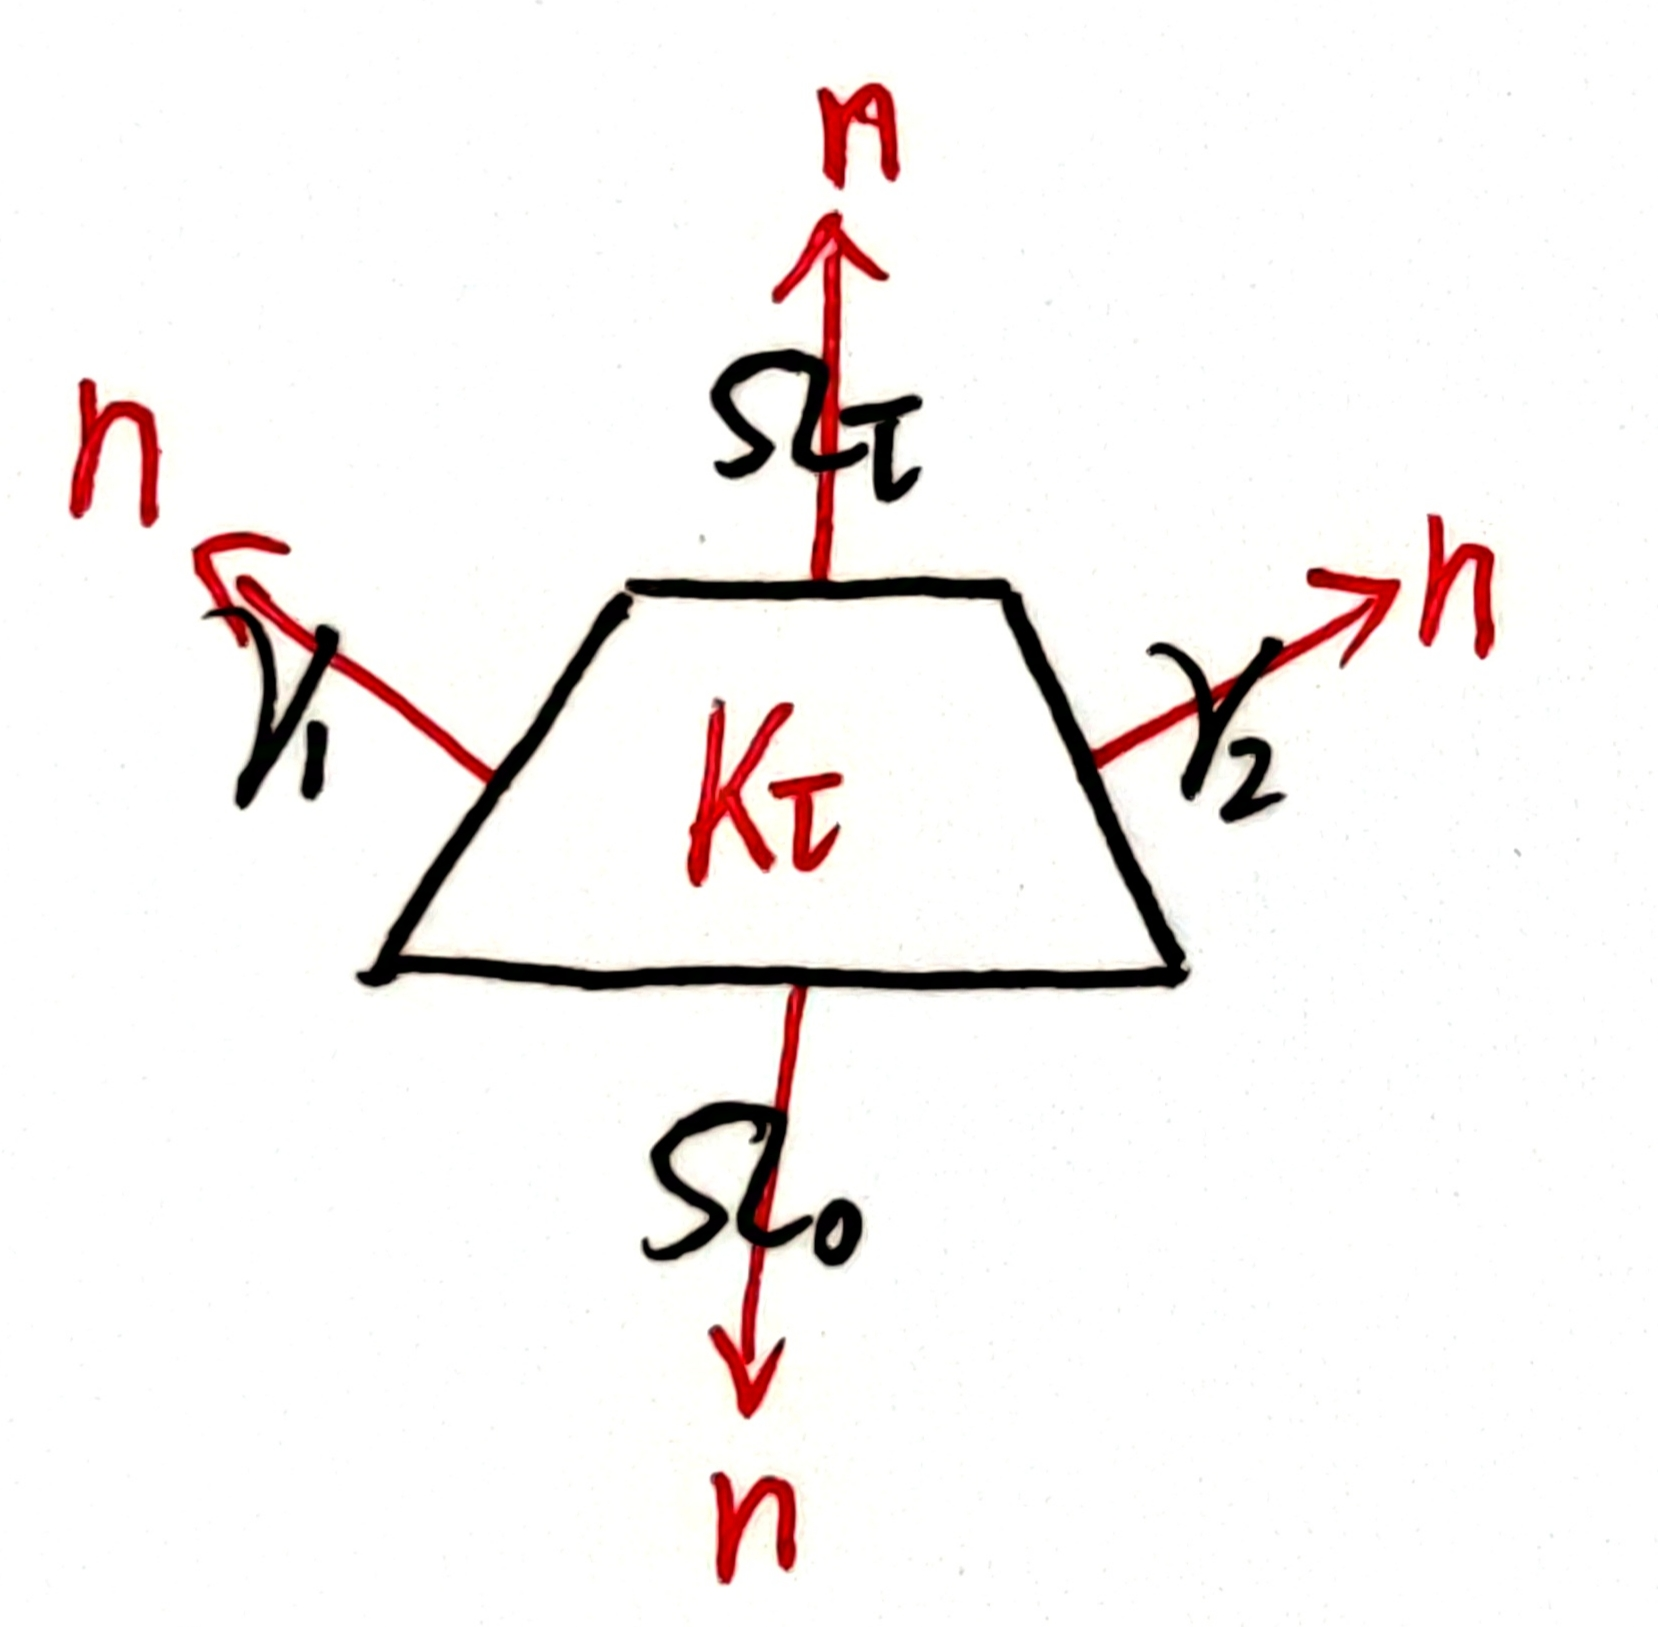
\includegraphics[width=0.5\linewidth]{figure/2.3-5}
						\caption{区域$K_\tau$ 各边记号及法向}
						\label{fig : 2.3-5}
					\end{minipage}
				\end{figure}
				
				经过简单的计算, 可得到各边法向$\vec{n} = (n_x , n_t)$ 为:
				\begin{align*}
					\begin{cases}
						\Omega_\tau : n_x = 0 , \,\, n_t = 1 \\
						\Omega_0 : n_x = 0 , \,\, n_t = -1 \\
						\gamma_1 : n_x = \dfrac{-1}{\sqrt{1 + c^2}} , \,\, n_t = \dfrac{c}{\sqrt{1 + c^2}} \\
						\gamma_2 : n_x = \dfrac{1}{\sqrt{1 + c^2}} , \,\, n_t = \dfrac{c}{\sqrt{1 + c^2}}
					\end{cases}
				\end{align*}
				\underline{\textbf{下面来构造能量不等式}}:\\
				Since $u_{tt} - c^2 u_{xx} = 0$ on $\R \times (0 , \infty)$, then
				\[ \int_{K_\tau} u_t (u_{tt} - c^2 u_{xx}) = 0 \]
				Since
				\begin{align*}
					\begin{cases}
						u_t \cdot u_{tt} = \dfrac{1}{2} \dfrac{\partial}{\partial t}u_{t}^2 \\
						u_t \cdot u_{xx} = \dfrac{\partial}{\partial x} (u_t \cdot u_x) - \dfrac{1}{2} \dfrac{\partial}{\partial t} u_{x}^2
					\end{cases}
				\end{align*}
				Hence by \textbf{Gauss-Green Theorem (Thm \ref{thm B.4.1})}, 
				\begin{align*}
					0 
					&= \int_{K_\tau} \left\{ \frac{1}{2} \frac{\partial}{\partial t} \big[ u_{t}^2 + c^2 u_{x}^2 \Big] - c^2 \dfrac{\partial}{\partial x} (u_t \cdot u_x) \right\} 
					= \int_{\partial K_\tau} \left\{ \frac{1}{2} ( u_{t}^2 + c^2 u_{x}^2 ) \cdot n_t - c^2 u_t u_x \cdot n_x \right\} \\
					&= \int_{\Omega_\tau} \frac{1}{2} [ u_{t}^2 + c^2 u_{x}^2 ] + 
					\int_{\Omega_0} -\frac{1}{2} [ u_{t}^2 + c^2 u_{x}^2 ] + 
					\int_{\gamma_1} \left\{ \frac{1}{2} [ u_{t}^2 + c^2 u_{x}^2 ] \cdot \frac{c}{\sqrt{1 + c^2}} - c^2 u_t u_x \cdot \Big( \frac{-1}{\sqrt{1 + c^2}} \Big) \right\} + \\
					&\int_{\gamma_2} \left\{ \frac{1}{2} [ u_{t}^2 + c^2 u_{x}^2 ] \cdot \frac{c}{\sqrt{1 + c^2}} - c^2 u_t u_x \cdot \frac{1}{\sqrt{1 + c^2}} \right\}
				\end{align*}
				对于上述等式, 将$\Omega_0$ 上的积分移至等号另一侧, 等式两边乘2. 
				\newpage
				Since $\Omega_0 \subset \R \times \{ t = 0 \}$, then
				\[ \int_{\Omega_0} [ u_{t}^2 + c^2 u_{x}^2 ] = \int_{\Omega_0} [ \psi^2 + c^2 \varphi_{x}^2 ] \]
				At the same time, 
				\begin{align*}
					\int_{\gamma_1} \left\{ \frac{1}{2} [ u_{t}^2 + c^2 u_{x}^2 ] \cdot \frac{c}{\sqrt{1 + c^2}} - c^2 u_t u_x \cdot \Big( \frac{-1}{\sqrt{1 + c^2}} \Big) \right\} 
					= \frac{c}{\sqrt{1 + c^2}} \cdot \int_{\gamma_1} (u_t + cu_x)^2
				\end{align*}
				Similarly, 
				\[ \int_{\gamma_2} \left\{ \frac{1}{2} [ u_{t}^2 + c^2 u_{x}^2 ] \cdot \frac{c}{\sqrt{1 + c^2}} - c^2 u_t u_x \cdot \frac{1}{\sqrt{1 + c^2}} \right\} 
				= \frac{c}{\sqrt{1 + c^2}} \cdot \int_{\gamma_2} (u_t - cu_x)^2 \]
				故进行上述移项操作后, 可得
				\begin{align*}
					\int_{\Omega_0} [ \psi^2 + c^2 \varphi_{x}^2 ] 
					&= \int_{\Omega_\tau} [ u_{t}^2 + c^2 u_{x}^2 ] 
					+ \frac{c}{\sqrt{1 + c^2}} \cdot \int_{\gamma_1} (u_t + cu_x)^2 
					+ \frac{c}{\sqrt{1 + c^2}} \cdot \int_{\gamma_2} (u_t - cu_x)^2 \\
					&\geq \int_{\Omega_\tau} [ u_{t}^2 + c^2 u_{x}^2 ]
				\end{align*}
				i.e.
				\begin{align}
					\int_{\Omega_0} [ \psi^2 + c^2 \varphi_{x}^2 ] \geq \int_{\Omega_\tau} [ u_{t}^2 + c^2 u_{x}^2 ] , \,\, \forall \tau \in [0 , t_0] , \,\, \forall (x_0 , t_0) \in \R \times (0 , \infty) \label{2.13}
				\end{align}
				
				\vspace*{1.5em}
				
				此即为\textbf{一维齐次波动方程的\underline{\textcolor{blue}{能量不等式}}}\footnote{对于一般的一维波动方程的\textbf{能量不等式}, 可见\textbf{附录\ref{appendix A} - Thm \ref{thm A.4.1}}. }, 积分$\int_{\Omega_\tau} [u_{t}^2 + c^2 u_{x}^2]$ 称为\underline{\textcolor{blue}{\textbf{能量积分}}}, 表示弦振动问题中弦段$\Omega_\tau$ 在$t$ 时刻的总能量. 下面利用该不等式来证明解的唯一性:
				
				\vspace*{1.5em}
				
				Suppose both $u_1 \,\, \& \,\, u_2$ are solutions. Then
				\begin{align*}
					\begin{cases}
						(u_1 - u_2)_{tt} - c^2 (u_1 - u_2)_{xx} = 0 , \,\, x \in \R , t > 0 \\
						(u_1 - u_2) \Big|_{t = 0} = 0 \\
						(u_1 - u_2)_{t} \Big|_{t = 0} = 0
					\end{cases}
				\end{align*}
				Then by \textbf{Energe Inequality}, 
				\[ 0 \geq \int_{\Omega_\tau} (u_1 - u_2)_{t}^2 + c^2 (u_1 - u_2)_{x}^2 , \,\, \forall \tau \in [0 , t_0] , \,\, \forall (x_0 , t_0) \in \R \times (0 , \infty) \]
				Thus
				\[ (u_1 - u_2)_t \equiv (u_1 - u_2)_x \equiv 0 \,\, \text{on} \,\, \R \times [0 , \infty) \]
				Hence
				\[ u_1 - u_2 \equiv C \,\, \text{for some} \,\, C \in \R \]
				Since $(u_1 - u_2) \Big|_{t = 0} = 0$, then $C = 0$. Therefore, $u_1 = u_2$. 
			\end{itemize}
		\end{proof}
	\end{thm}

\newpage

\subsection{一维波动方程的特征线法 (上半空间)}
	根据\textbf{一维齐次波动方程的解 (Thm \ref{thm 2.3.1})}, 可得到齐次波动方程的解为
	\[ u(x , t) = \frac{1}{2} \Big[ \varphi(x + ct) + \varphi(x - ct) \Big] + \frac{1}{2c} \int_{x - ct}^{x + ct} \psi(\xi) \, d\xi \]
	令$\varphi = 0$, 得到定解问题(\ref{A.2}) 的解为
	\[ M_{\psi} = \frac{1}{2c} \int_{x - ct}^{x + ct} \psi(\xi) \, d\xi \]
	从而对于非齐次问题
	\begin{align*}
		\begin{cases}
			\dfrac{\partial^2 u}{\partial t^2} - c^2 \dfrac{\partial^2 u}{\partial x^2} = f(x , t) , \,\, x \in \R , t > 0 \\
			u \Big|_{t = 0} = 0 \\
			u_{t} \Big|_{t = 0} = 0
		\end{cases}
	\end{align*}
	根据\textbf{一维波动方程的Duhamel原理 (齐次化原理, Thm \ref{thm A.3.1})}, 得到其解为
	
	\begin{align*}
		u(x , t) 
		= \int_{0}^t M_{f_\tau}(x , t - \tau) \, d\tau 
		&= \frac{1}{2c} \int_{0}^t \Big( \int_{x - c\tau}^{x + c\tau} f(\xi , t - \tau) \, d\xi \Big) \, d\tau \\
		&= \frac{1}{2c} \int_{0}^t \Big( \int_{x - c(t - \tau)}^{x + c(t - \tau)} f(\xi , \tau) \, d\xi \Big) \, d\tau
	\end{align*}
	
	\vspace*{2em}
	
	where $f_{\tau} = f(x , \tau)$. 根据\textbf{线性PDE的叠加原理 (Thm \ref{thm A.2.1})}, 可得到上半空间$\R \times [0 , \infty)$ 上一般的一维波动方程的初值问题的解, 即下面给出的定理. 
	
	\newpage
	
	\begin{thm}\label{thm 2.3.2}
		\textbf{[一维波动方程解的存在唯一性, 上半空间, D'Alembert, 能量不等式]}. \\
		If $\varphi \in C^2(\R)$, $\psi \in C^1(\R)$, $f \in C^1 \Big( \R \times [0 , \infty) \Big)$, then for the Cauchy Problem (\ref{2.10})
		\begin{align*}
			\begin{cases}
				\dfrac{\partial^2 u}{\partial t^2} - c^2 \dfrac{\partial^2 u}{\partial x^2} = f(x , t) , \,\, x \in \R , t > 0 \\
				u \Big|_{t = 0} = \varphi(x) \\
				u_t \Big|_{t = 0} = \psi(x)
			\end{cases}
		\end{align*}
		It has a unique solution $u \in C^2 \Big( \R \times (0 , \infty) \Big) \cap C^1 \Big( \R \times [0 , \infty) \Big)$:
		\begin{align}
			u(x , t) = \frac{1}{2} \Big[ \varphi(x + ct) + \varphi(x - ct) \Big] + \frac{1}{2c} \int_{x - ct}^{x + ct} \psi(\xi) \, d\xi + \frac{1}{2c} \int_{0}^t \Big( \int_{x - c(t - \tau)}^{x + c(t - \tau)} f(\xi , \tau) \, d\xi \Big) \, d\tau \label{2.14}
		\end{align}
		which is called the \underline{\textcolor{blue}{\textbf{D'Alembert Formula}}}. 
		
		\vspace*{4em}
		
		\begin{rmk}
			\begin{itemize}
				\item 对于解的\textbf{存在性}, 可根据\textbf{一维齐次波动方程解的存在唯一性 (Thm \ref{thm 2.3.1})}与\textbf{线性PDE的叠加原理 (Thm \ref{thm A.2.1})}, 得到解的形式的推导过程. 再代入原问题证明其是原方程的解. 
				
				\vspace*{2em}
				
				\item 对于解的\textbf{唯一性}, 可根据\textbf{一维波动方程的能量不等式 (Thm \ref{thm A.4.1})}, 类比\textbf{一维齐次波动方程解的存在唯一性 (Thm \ref{thm 2.3.1})} 中唯一性的证明得到. 
			\end{itemize}
		\end{rmk}
	\end{thm}

\newpage

\subsection{一维波动方程的特征线法 (半无界问题)}
	对于\underline{\textbf{半无界区域 $[0 , \infty) \times [0 , \infty)$}}上考虑一般的一维波动方程的初值问题, 对于$x = 0$ 处所给的初值条件, 一般有以下两种:
	
	\begin{align*}
		\begin{cases}
			\dfrac{\partial^2 u}{\partial t^2} - c^2 \dfrac{\partial^2 u}{\partial x^2} = f(x , t) , \,\, x > 0 , t > 0 \\
			u \Big|_{t = 0} = \varphi(x) \\
			u_t \Big|_{t = 0} = \psi(x) \\
			u \Big|_{x = 0} = g(t)
		\end{cases} , \hspace*{2em} 
		\begin{cases}
			\dfrac{\partial^2 u}{\partial t^2} - c^2 \dfrac{\partial^2 u}{\partial x^2} = f(x , t) , \,\, x > 0 , t > 0 \\
			u \Big|_{t = 0} = \varphi(x) \\
			u_t \Big|_{t = 0} = \psi(x) \\
			u_x \Big|_{x = 0} = g(t)
		\end{cases}
	\end{align*}
	
	\vspace*{2em}
	
	\hspace*{-1.95em}上述两个问题分别称为\underline{\textcolor{blue}{\textbf{第一类边界问题}}}和\underline{\textcolor{blue}{\textbf{第二类边界问题}}}. 对于这两种问题的一般形式, 分别作变换
	\[ v(x , t) = u(x , t) - g(t) \hspace*{1em} , \hspace*{1em} v(x , t) = u(x , t) - x \cdot g(t) \]
	可将各自在$x = 0$ 处的边值条件变为0, 即$u \Big|_{x = 0} = 0$ 及$u_x \Big|_{x = 0} = 0$. 故只需考虑如下齐次边界问题:
	
	\begin{align*}
		\begin{cases}
			\dfrac{\partial^2 u}{\partial t^2} - c^2 \dfrac{\partial^2 u}{\partial x^2} = f(x , t) , \,\, x > 0 , t > 0 \\
			u \Big|_{t = 0} = \varphi(x) \\
			u_t \Big|_{t = 0} = \psi(x) \\
			u \Big|_{x = 0} = 0
		\end{cases} , \hspace*{2em} 
		\begin{cases}
			\dfrac{\partial^2 u}{\partial t^2} - c^2 \dfrac{\partial^2 u}{\partial x^2} = f(x , t) , \,\, x > 0 , t > 0 \\
			u \Big|_{t = 0} = \varphi(x) \\
			u_t \Big|_{t = 0} = \psi(x) \\
			u_x \Big|_{x = 0} = 0
		\end{cases}
	\end{align*}
	
	\vspace*{2em}
	
	\hspace*{-1.95em}对于一维实轴$\R$ 上的光滑函数$h(x)$, 若$h$ 为奇函数, 则有$h \Big|_{x = 0} = 0$;若$h$ 为偶函数, 则$h_x \Big|_{x = 0} = 0$. 基于该想法, 我们对上述两种边界问题, 分别采用\underline{\textcolor{blue}{\textbf{奇延拓}}}和\underline{\textcolor{blue}{\textbf{偶延拓}}}的方法进行求解, 即将$f , \varphi , \psi$ 延拓至整个上半空间 ($f$ 为$\R \times (0 , \infty)$, $\varphi , \psi$ 为$\R$)上, 使得$f , \varphi , \psi$ 均关于$x$ 称为奇 (偶)函数. 
	
	\newpage
	
	\begin{thm}\label{thm 2.3.3}
		\textbf{[一维波动方程解的存在唯一性, 半无界问题, D'Alembert, 第一类边界]}. \\
		If $\varphi \in C^2[0 , \infty)$, $\psi \in C^1[0 , \infty]$, $f \in C^1 \Big( [0 , \infty) \times [0 , \infty) \Big)$, then for the Cauchy Problem (\ref{2.10})
		\begin{align*}
			\begin{cases}
				\dfrac{\partial^2 u}{\partial t^2} - c^2 \dfrac{\partial^2 u}{\partial x^2} = f(x , t) , \,\, x > 0 , t > 0 \\
				u \Big|_{t = 0} = \varphi(x) \\
				u_t \Big|_{t = 0} = \psi(x) \\
				u \Big|_{x = 0} = 0
			\end{cases}
		\end{align*}
		此时可对$f , \varphi , \psi$ 进行奇延拓:
		\begin{align*}
			\overline{f}(x , t) = 
			\begin{cases}
				f(x  ,t) , \,\, x \geq 0 , t \geq 0 \\
				-f(-x , t) , \,\, x < 0 , t \geq 0
			\end{cases} , \hspace*{1em}
			\overline{\varphi}(x) = 
			\begin{cases}
				\varphi(x) , \,\, x \geq 0 \\
				-\varphi(-x) , \,\, x < 0
			\end{cases} , \hspace*{1em}
			\overline{\psi}(x) = 
			\begin{cases}
				\psi(x) , \,\, x \geq 0 \\
				-\psi(-x) , \,\, x < 0
			\end{cases}
		\end{align*}
		Then for the new Cauchy Problem
		\begin{align*}
			\begin{cases}
				\dfrac{\partial^2 u}{\partial t^2} - c^2 \dfrac{\partial^2 u}{\partial x^2} = \overline{f}(x , t) , \,\, x \in \R , t > 0 \\
				u \Big|_{t = 0} = \overline{\varphi}(x) \\
				u_t \Big|_{t = 0} = \overline{\psi}(x) \\
				u \Big|_{x = 0} = 0
			\end{cases}
		\end{align*}
		
		\vspace*{1em}
		
		\hspace*{-1.95em}It has a unique solution $\overline{u} \in C^2 \Big( \R \times (0 , \infty) \Big) \cap C^1 \Big( \R \times [0 , \infty) \Big)$:
		\begin{align}
			\overline{u}(x , t) = \frac{1}{2} \Big[ \overline{\varphi}(x + ct) + \overline{\varphi}(x - ct) \Big] + \frac{1}{2c} \int_{x - ct}^{x + ct} \overline{\psi}(\xi) \, d\xi + \frac{1}{2c} \int_{0}^t \Big( \int_{x - c(t - \tau)}^{x + c(t - \tau)} \overline{f}(\xi , \tau) \, d\xi \Big) \, d\tau \label{2.15}
		\end{align}
		
		\vspace*{1em}
		
		\hspace*{-1.95em}which is called the \underline{\textcolor{blue}{\textbf{D'Alembert Formula}}}. In response to the origin problem, it has the unique solution $u \in C^2 \Big( (0 , \infty) \times (0 , \infty) \Big) \cap C^1 \Big( [0 , \infty) \times [0 , \infty) \Big)$, which can be represented by:
		
		\vspace*{1em}
		
		\hspace*{-1.95em}When $x > ct$, 
		\[ u(x , t) = \frac{1}{2} \Big[ \varphi(x + ct) + \varphi(x - ct) \Big] + \frac{1}{2c} \int_{x - ct}^{x + ct} \psi(\xi) \, d\xi + \frac{1}{2c} \int_{0}^t \Big( \int_{x - c(t - \tau)}^{x + c(t - \tau)} f(\xi , \tau) \, d\xi \Big) \, d\tau \]
		When $x < ct$, 
		\begin{align*}
			u(x , t) 
			= &\frac{1}{2} \Big[ \varphi(x + ct) - \varphi(ct - x) \Big] 
			+ \frac{1}{2c} \int_{ct - x}^{x + ct} \psi(\xi) \, d\xi \\
			+ &\frac{1}{2c} \left[ \int_{t - \tfrac{x}{c}}^t \Big( \int_{x - c(t - \tau)}^{x + c(t - \tau)} f(\xi , \tau) \, d\xi \Big) \, d\tau + \int_{0}^{t - \tfrac{x}{c}} \Big( \int_{c(t - \tau) - x}^{x + c(t - \tau)} f(\xi , \tau) \, d\xi \Big) \, d\tau \right]
		\end{align*}
		
		\newpage
		
		\begin{rmk}
			\begin{itemize}
				\item 解的\textbf{存在唯一性}可类似\textbf{Thm \ref{thm 2.3.2}} 得到, 其中\textbf{唯一性}可在半无界区域上利用能量不等式证明\footnote{详细论述可参考:\textbf{《数学物理方程讲义 (第二版)》--  姜礼尚、陈亚浙、刘西垣、易法槐} -- $\S 2.2.5$ 半无界问题. }.
				
				\vspace*{2em}
				
				\item 对于\textbf{第二类边界问题}, 将$f , \varphi , \psi$ 进行\textbf{偶延拓}, 
				\begin{align*}
					\overline{f}(x , t) = 
					\begin{cases}
						f(x  ,t) , \,\, x \geq 0 , t \geq 0 \\
						f(-x , t) , \,\, x < 0 , t \geq 0
					\end{cases} , \hspace*{1em}
					\overline{\varphi}(x) = 
					\begin{cases}
						\varphi(x) , \,\, x \geq 0 \\
						\varphi(-x) , \,\, x < 0
					\end{cases} , \hspace*{1em}
					\overline{\psi}(x) = 
					\begin{cases}
						\psi(x) , \,\, x \geq 0 \\
						\psi(-x) , \,\, x < 0
					\end{cases}
				\end{align*}
				可类似得到\textbf{解的存在唯一性}. 
			\end{itemize}
		\end{rmk}
	\end{thm}

\newpage

\subsection{Sturm-Liouville Problem}
	这一小节我们将对于\textbf{二阶常微分方程}
	\[ X^{''} + \lambda X = 0 , \,\, x \in (0 , l) \]
	的\textbf{Sturm-Liouville问题}给出相关结论. 这是下一节\textbf{分离变量法}的理论基础. 首先给出一些基础概念的定义. 
	
	\vspace*{1em}
	
	\begin{defn}\label{def 2.3.2}
		对于ODE齐次边值问题 
		\begin{align}
			\begin{cases}
				X^{''} + \lambda X = 0 , \,\, x \in (0 , l) \\
				-\alpha_1 X^{'}(0) + \beta_1 X(0) = 0 \\
				\alpha_2 X^{'}(l) + \beta_2 X(l) = 0
			\end{cases} , \,\, 
			\alpha_i , \beta_i \geq 0 , \,\, \alpha_i + \beta_i \neq 0 , \,\, \forall i = 1 , 2 \label{2.16}
		\end{align}
		使其具有非零解的$\lambda$ 称为该边值问题的\underline{\textcolor{blue}{\textbf{特征值}}}, 对应的非零解$X(x)$ 称为这个特征值对应的\underline{\textcolor{blue}{\textbf{特征函数}}}. 而寻求方程(\ref{2.16}) 的所有特征值和特征函数的问题称为\underline{\textcolor{blue}{\textbf{Sturm-Liouville 问题}}}或\underline{\textcolor{blue}{\textbf{特征值问题}}}. 
	\end{defn}
	
	\vspace*{6em}
	
	下面我们不加证明地给出有关二阶ODE的\textbf{Sturm-Liouville问题}的相关结论. 
	
	\newpage
	
	\begin{thm}\label{thm 2.3.4}
		\textbf{[Sturm-Liouville]}\footnote{定理的部分证明可参考:\textbf{《数学物理方程讲义 (第二版)》--  姜礼尚、陈亚浙、刘西垣、易法槐} -- $\S 2.4$ 定理4.1. }. \\
		考虑$[0 , l]$ 上的Sturm-Liouville问题 (\ref{2.16})
		\begin{align*}
			\begin{cases}
				X^{''} + \lambda X = 0 , \,\, x \in (0 , l) \\
				-\alpha_1 X^{'}(0) + \beta_1 X(0) = 0 \\
				\alpha_2 X^{'}(l) + \beta_2 X(l) = 0
			\end{cases} , \,\, 
			\alpha_i , \beta_i \geq 0 , \,\, \alpha_i + \beta_i \neq 0 , \,\, \forall i = 1 , 2 
		\end{align*}
		其具有如下性质:
		
		\vspace*{1em}
		
		\begin{enumerate}
			\item [(\rmnum{1})] 其有可数个非负实特征值, 每个特征值单重, 特别当$\beta_1 + \beta_2 > 0$ 时, 所有特征值均为正数. 
			
			\vspace*{3em}
			
			\item[(\rmnum{2})] 所有特征值组成一个严格单调递增、以无穷远点为聚点的序列 (无有限聚点):
			\[ 0 \leq \lambda_1 < \lambda_2 < \cdots < \lambda_n < \cdots , \,\, \lim_{n \to \infty}\lambda_n = \infty \]
			
			\vspace*{3em}
			
			\item[(\rmnum{3})] 对于所有的特征值$\{ \lambda_n \}_{n = 1}^{\infty}$ 对应的特征函数$\{ X_{n} \}_{n = 1}^{\infty}$, 其构成了Hilbert空间$L^{2}[0 , l]$ 上的一组\textbf{完备正交系}\footnote{在\textbf{《泛函分析讲义》 -- 张恭庆、林源渠} 一书中称为\underline{\textbf{封闭的正交集}}. }, 即
			\[ \int_{0}^l X_{k}(x) X_{l}(x) \, dx = 0 , \,\, \forall k \neq l \]
			且对于$\forall f \in L^2[0 , l]$, $\exists C_n \in \R$, $\st$
			\[ f(x) = \sum_{n = 1}^{\infty} C_n X_n(x) \]
			where
			\[ C_n = \frac{(f , X_n)}{(X_n , X_n)} = \frac{\int_{0}^l f(x) X_n(x) \, dx}{\int_{0}^l X_{n}^2(x) \, dx} , \,\, \forall n \in \N \]
			\[  \]
		\end{enumerate}
	\end{thm}

\newpage

\subsection{一维齐次波动方程的分离变量法 (混合问题)}
	在\underline{\textbf{混合区域 $[0 , l] \times [0 , \infty)$}}上考虑一维齐次波动方程的初值问题:
	\begin{align}
		\begin{cases}
			\dfrac{\partial^2 u}{\partial t^2} - c^2 \dfrac{\partial^2 u}{\partial x^2} = 0 , \,\, x \in (0 , l) , t > 0 \\
			u \Big|_{t = 0} = \varphi(x) \\
			u_t \Big|_{t = 0} = \psi(x) \\
			u(0 , t) = u(l , t) = 0
		\end{cases} \label{2.17}
	\end{align}
	我们既可以类似$\S$2.3 节\textbf{Thm \ref{thm 2.3.3}}, 将$u$ 延拓为整个上半空间的函数, 再利用\textbf{D'Alembert 公式 (Thm \ref{thm 2.3.2})}求解 (在\textbf{Thm \ref{thm 2.3.5}} 注解中会讨论);但也可通过下面介绍的\textbf{分离变量法}进行求解. 且该方法还可推广至\textbf{热方程 (Heat Equation)的混合问题}等问题的求解中. 
	
	\vspace*{1em}
	
	\begin{figure}[thbp!]
		\centering
		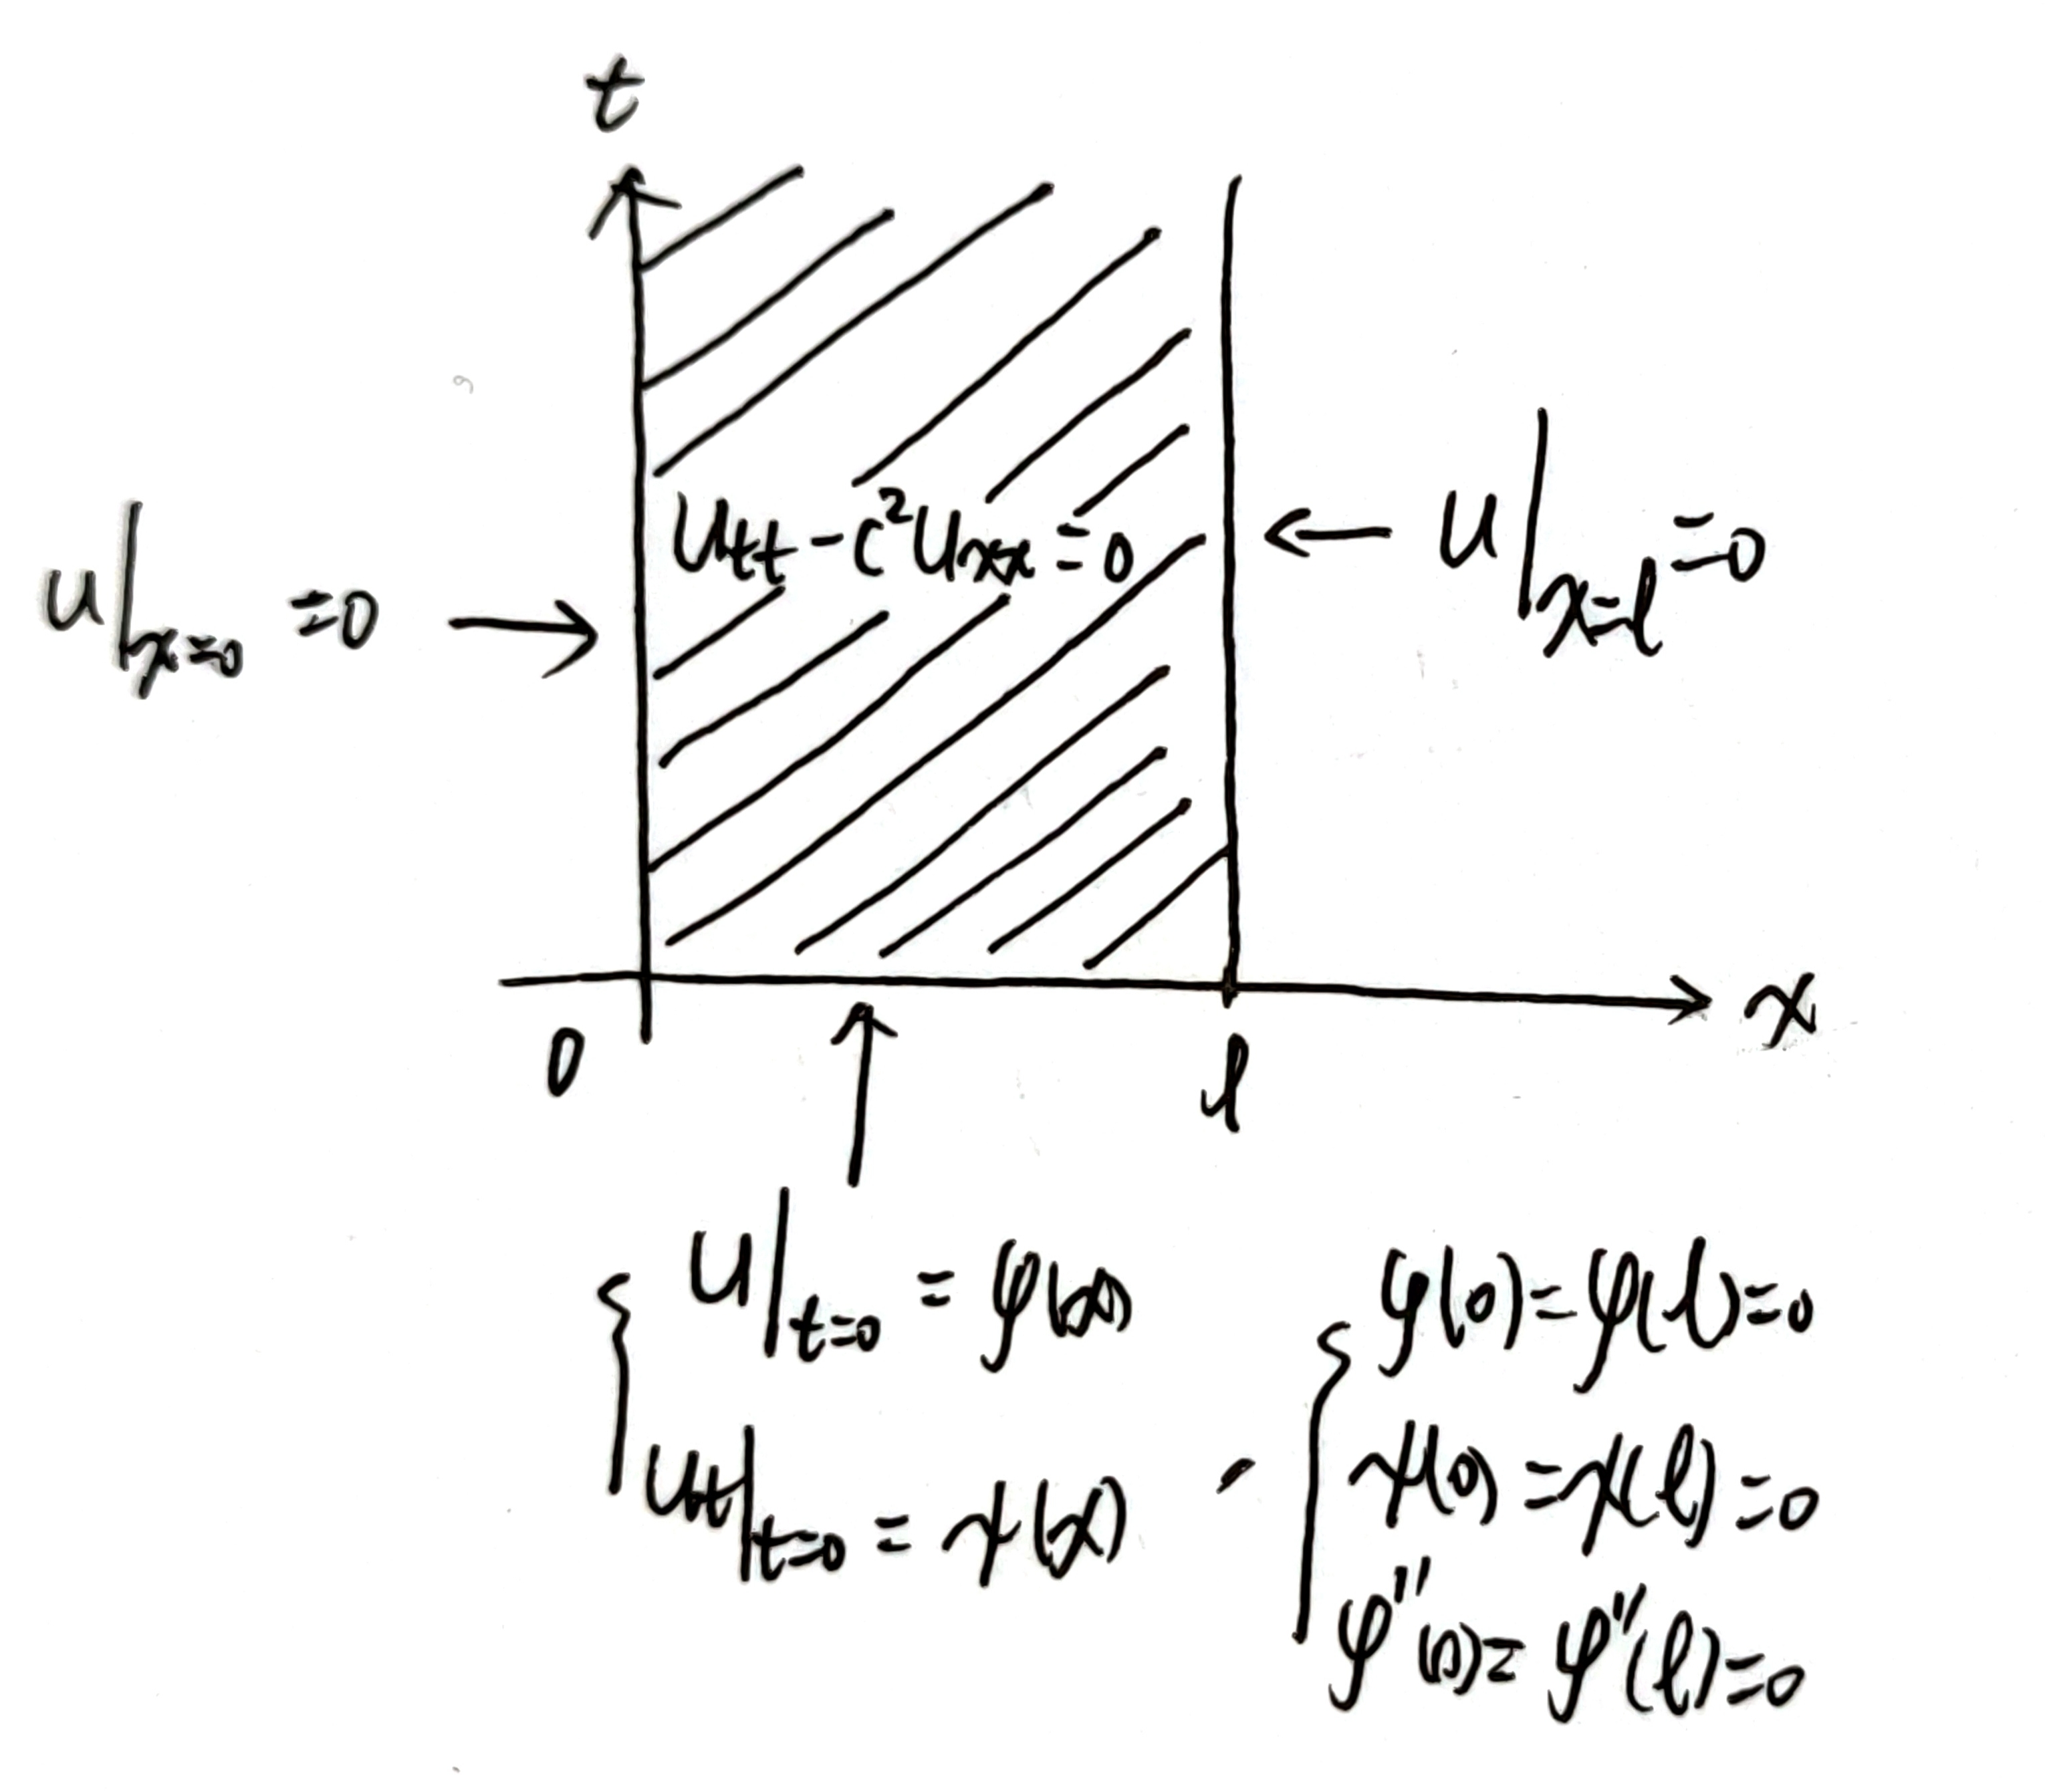
\includegraphics[width=0.6\linewidth]{figure/2.3-7}
		\caption{一维齐次波动方程的混合问题}
		\label{pic : 2.3-7} % 添加图像引用标签
	\end{figure}
	
	\vspace*{2em}
	
	下面给出\textbf{分离变量法}求解一维齐次波动方程混合问题的\textbf{解的存在唯一性}讨论. 
	
	\newpage
	
	\begin{thm}\label{thm 2.3.5}
		\textbf{[一维齐次波动方程, 混合问题, 分离变量法]}. \\
		Suppose $\varphi \in C^3[0 , l]$, $\psi \in C^2[0 , l]$, 且$\varphi(x) , \psi(x)$ 满足相容性条件:
		\begin{align*}
			\begin{cases}
				\varphi(0) = \varphi(l) = 0 \\
				\psi(0) = \psi(l) = 0 \\
				\varphi^{''}(0) = \varphi^{''}(l) = 0
			\end{cases}
		\end{align*}
		Then for the homogenuous problem (\ref{2.17})
		\begin{align*}
			\begin{cases}
				\dfrac{\partial^2 u}{\partial t^2} - c^2 \dfrac{\partial^2 u}{\partial x^2} = 0 , \,\, x \in (0 , l) , t > 0 \\
				u \Big|_{t = 0} = \varphi(x) \\
				u_t \Big|_{t = 0} = \psi(x) \\
				u(0 , t) = u(l , t) = 0
			\end{cases}
		\end{align*}
		The formula
		\begin{align}
			u(x) = \sum_{n = 1}^{\infty} \left( A_n \sin \frac{cn\pi}{l} t + B_n \cos \frac{cn\pi}{l} t \right) \sin \frac{n\pi}{l} x \label{2.18}
		\end{align}
		where 
		\begin{align}
			\begin{dcases}
				A_n = \dfrac{2}{cn\pi} \int_{0}^l \psi(x) \sin \frac{n\pi}{l} x \, dx \\
				B_n = \dfrac{2}{l} \int_{0}^l \varphi(x) \sin \frac{n\pi}{l} x \, dx 
			\end{dcases}, \,\, \forall n \in \N \label{2.19}
		\end{align}
		defines a function $u \in C^{2}\Big( [0 , l] \times [0 , \infty) \Big)$ and gives the unique solution of (\ref{2.17}) in $C^{2}\Big( [0 , l] \times [0 , \infty) \Big)$. 
		
		\vspace*{6em}
		
		\begin{rmk}
			事实上, 对于问题 (\ref{2.17}), 我们可以采取与\textbf{Thm \ref{thm 2.3.3}} 类似的\textbf{对称开拓法}, 并结合\textbf{D'Alembert公式}求解. 根据\textbf{Thm \ref{thm 2.3.3}}, 此方法关于$\varphi , \psi$ 的光滑性可进一步减弱为
			\[ \varphi \in C^2[0 , l] , \,\, \psi \in C^1[0 , l] \]
			\textbf{对称开拓法}即定义周期为$2l$ 的周期奇函数$\Phi , \Psi$, 使其分别成为$\varphi , \psi$ 的延拓, 具体为
			\begin{align*}
				\begin{cases}
					\Phi(x) = -\Phi(-x) , \,\, \Phi(x) = \Phi(x + 2l) , \,\, x \in \R \\
					\Phi(x) = \varphi(x) , \,\, x \in [0 , l]
				\end{cases} , \,\, 
				\begin{cases}
					\Psi(x) = -\Psi(-x) , \,\, \Psi(x) = \Psi(x + 2l) , \,\, x \in \R \\
					\Psi(x) = \psi(x) , \,\, x \in [0 , l]
				\end{cases}
			\end{align*}
			可以证明, 在$\varphi \in C^3 , \psi \in C^2$ 的条件下, 这两种方法得到的$u$ 相等. 
		\end{rmk}
		
		\newpage
		
		\begin{proof}
			\begin{itemize}
				\item \textbf{存在性}:\textbf{[\uwave{分离变量法}求解过程]}
				\begin{center}
					\textbf{[思路:先证明若有特解可满足变量分离, 则解满足上述形式;(Step 1:P38 - 40)\\
						再将该特解$u$ 回代至原问题, 证明它是解 (Step 2:P40 - 44)]}. 
				\end{center}
				
				\begin{enumerate}
					\item[\textbf{Step 1}]. \underline{\textbf{先证明若有特解可满足变量分离, 则解满足上述形式}}:\\
					假设非零特解$u(x , t) \in C^2\Big( [0 , l] \times [0 , \infty) \Big)$ 具有变量分离形式, i.e. $\exists X(x) , T(t)$, $\st$
					\[ u(x , t) = X(x) T(t) \]
					Since 
					\[ u_{tt} - c^2 u_xx = 0 \,\,\,\, \text{and} \,\,\,\, u\Big|_{x = 0} = u \Big|_{x = l} = 0 \]
					Then 
					\[ XT^{''} - c^2 X^{''}T = 0 \,\,\,\, \text{and} \,\,\,\, X(0) T(t) = X(l)T(t) = 0 , \,\, \forall t > 0 \]
					i.e.
					\[ \frac{X^{''}}{X} = \frac{T^{''}}{c^2 T} \]
					由于等式左侧仅为$x$ 的函数, 右侧为$t$ 的函数, 因此该等式恒为定值, 记为$-\lambda$, 则有
					\begin{align*}
						T^{''} + c^2 \lambda T &= 0 , \,\, t > 0 \\
						X^{''} + \lambda X &= 0 , \,\, x \in (0 , l)
					\end{align*}
					由于$u(x , t)$ 为非零特解, $X(0) T(t) = X(l)T(t) = 0$, 因此$X(0) = X(l) = 0$. 从而$X$ 满足
					\begin{align}
						\begin{cases}
							X^{''} + \lambda X = 0 , \,\, x \in (0 , l) \\
							X(0) = 0 \\
							X(l) = 0
						\end{cases} \label{2.20}
					\end{align}
					故根据\textbf{Def \ref{def 2.3.2}}, 求解$X(x)$ 即为求解上述\textbf{Sturm-Liouville问题}. 根据\textbf{一阶常系数线性ODE的求解 (Thm \ref{thm B.5.1})}, 得到上述ODE的通解为
					\[ X(x) = C_1 \sin \sqrt{\lambda} x + C_2 \cos \sqrt{\lambda} x \]
					结合边界条件$X(0) = X(l) = 0$, 得到
					\[ C_2 = 0 , \,\, C_1 \sin \sqrt{\lambda} \, l = 0 \]
					由于$u \not\equiv 0$, $X \not\equiv 0$, 因此$C_1 \neq 0$, $\sin \sqrt{\lambda} \, l = 0$. 从而该Sturm-Liouville问题所有可能的特征值为
					\[ \lambda = \left( \frac{n\pi}{l} \right)^2 , \,\, n = 0 , 1 , 2 , \cdots \]
					根据\textbf{Sturm-Liouville问题的性质 (Thm \ref{thm 2.3.4})}, 结合该方程, 可得到其所有的特征值及对应特征函数为
					\begin{align*}
						\lambda_n = \left( \frac{n \pi}{l} \right)^2 , \,\, X_n(x) = C \sin \frac{n\pi}{l}x , \,\, n = 1 , 2 , \cdots
					\end{align*}
					通过求解ODE
					\[ T^{''} + c^2 \lambda_n T = 0 , \,\, t > 0 , \,\, \forall n \in \N \]
					得到
					\[ T_n(t) = A_n \sin \frac{cn\pi}{l} t + B_n \cos \frac{cn\pi}{l} t , \,\, \forall n \in \N \]
					即可得到满足方程$u_{tt} - c^2 u_{xx} = 0$ 与边界条件$u\Big|_{x = 0} = u \Big|_{x = l} = 0$ 的函数$u_n$
					\[ u_n(x , t) = X_n(x) T_n(t) = \left( A_n \sin \frac{cn\pi}{l} t + B_n \cos \frac{cn\pi}{l} t \right) \sin \frac{n \pi}{l} x , \,\, \forall n \in \N \]
					Let 
					\begin{align*}
						u(x , t) 
						\coloneqq \sum_{n = 1}^{\infty} u_{n}(x , t) 
						= \sum_{n = 1}^{\infty} \left( A_n \sin \frac{cn\pi}{l} t + B_n \cos \frac{cn\pi}{l} t \right) \sin \frac{n \pi}{l} x 
					\end{align*}
					由于我们此时是求形式解, 因此不妨假设求和、求导、极限均可交换次序. 若上述定义的$u(x , t)$ 为所需特解, 则满足问题 (\ref{2.17}) 的边界条件, 即
					\[ u\Big|_{t = 0} = \varphi(x) , \,\, u_t \Big|_{t = 0} = \psi(x) \]
					i.e.
					\begin{align*}
						\varphi(x) &= u\Big|_{t = 0} = \sum_{n = 1}^{\infty} B_n \sin \frac{n\pi}{l} x \\
						\psi(x) &= u_t \Big|_{t = 0} = \sum_{n = 1}^{\infty} \frac{cn\pi}{l} A_n \sin \frac{n\pi}{l} x
					\end{align*}
					根据\textbf{Sturm-Liouville问题的性质 (Thm \ref{thm 2.3.4})}, Sturm-Liouville问题 (\ref{2.20}) 的所有特征函数$\{ X_n(x) \}_{n = 1}^{\infty} \subset L^2[0 , l]$ 构成了Hilbert空间$L^2[0 , l]$ 的一组完备正交系. 又因为$\varphi \in C^3[0 , l]$, $\psi \in C^2[0 , l]$ 在$[0 , l]$ 上连续, 所以$\varphi , \psi \in L^2[0 , l]$. Thus 
					\begin{align*}
						\varphi(x) &= \sum_{n = 1}^{\infty} \varphi_n X_n(x) = \sum_{n = 1}^{\infty} \varphi_n \sin \frac{n\pi}{l} x \\
						\psi(x) &= \sum_{n = 1}^{\infty} \psi_n X_n(x) = \sum_{n = 1}^{\infty} \psi_n \sin \frac{n\pi}{l} x
					\end{align*}
					where $\forall n \in \N$
					\begin{align*}
						\varphi_n &= \frac{(\varphi , X_n)}{(X_n , X_n)} = \frac{\int_{0}^l \varphi(x) \sin \dfrac{n\pi}{l} x \, dx}{\int_{0}^l \sin^2 \dfrac{n\pi}{l} x \, dx} = \frac{2}{l} \int_{0}^l \varphi(x) \sin \dfrac{n\pi}{l} x \, dx \\
						\psi_n &= \frac{(\varphi , X_n)}{(X_n , X_n)} = \frac{\int_{0}^l \varphi(x) \sin \dfrac{n\pi}{l} x \, dx}{\int_{0}^l \sin^2 \dfrac{n\pi}{l} x \, dx} = \frac{2}{l} \int_{0}^l \psi(x) \sin \dfrac{n\pi}{l} x \, dx
					\end{align*}
					Take
					\begin{align*}
						A_n &= \frac{2}{cn\pi} \int_{0}^l \psi(x) \sin \frac{n\pi}{l} x \, dx \\
						B_n &= \frac{2}{l} \int_{0}^l \varphi(x) \sin \dfrac{n\pi}{l} x \, dx
					\end{align*}
					因此若满足变量分离的特解存在, 则其形式为 (\ref{2.18})
					\begin{align*}
						u(x , t) = \sum_{n = 1}^{\infty} \left( A_n \sin \frac{cn\pi}{l} t + B_n \cos \frac{cn\pi}{l} t \right) \sin \frac{n\pi}{l} x
					\end{align*}
					
					\vspace*{4em}
					
					\item[\textbf{Step 2}]. \underline{\textbf{证明上述定义的$u(x , t)$ 是原问题的解}}:\\
					要证明上述定义的$u(x , t)$ 是原问题 (\ref{2.17}) 的解, 将其代入各条件, 即证
					\begin{align*}
						&(1) . \hspace*{2em} L\sum_{n = 1}^{\infty} u_n = \sum_{n = 1}^{\infty} Lu_n \\
						&(2) . \hspace*{2em} \lim_{x \to 0} \sum_{n = 1}^{\infty} u_n = \sum_{n = 1}^{\infty} \lim_{x \to 0} u_n , \,\, \lim_{x \to l} \sum_{n = 1}^{\infty} u_n = \sum_{n = 1}^{\infty} \lim_{x \to l} u_n \\
						&(3) . \hspace*{2em} \lim_{t \to 0} \sum_{n = 1}^{\infty} u_n = \sum_{n = 1}^{\infty} \lim_{t \to 0} u_n \\
						&(4) . \hspace*{2em} \lim_{t \to 0} \frac{\partial}{\partial t} \sum_{n = 1}^{\infty} u_n = \sum_{n = 1}^{\infty} \lim_{t \to 0} \frac{\partial}{\partial t} u_n
					\end{align*}
					where $L = \dfrac{\partial^2}{\partial t^2} - c^2 \dfrac{\partial^2}{\partial x^2}$. 而满足上述条件, 只需证明
					\[ \sum_{n = 1}^{\infty} u_n , \,\, \sum_{n = 1}^{\infty} Du_n , \,\, \sum_{n = 1}^{\infty} D^2 u_n \]
					一致收敛. 下面分别进行证明. 
					
					\newpage
					
					\begin{enumerate}
						\item[\textbf{(\rmnum{1})}]\underline{\textbf{$\overset{\infty}{\underset{n = 1}{\sum}} u_n$ 一致收敛}}:注意到$u_n = X_n T_n$. \\
						根据上述讨论, 
						\begin{align*}
							T_n(x) = \frac{l \cdot \psi_n}{cn\pi} \sin \frac{cn\pi}{l} t + \varphi_n \cos \frac{cn\pi}{l} t
						\end{align*}
						根据分部积分公式, 
						\begin{align*}
							\varphi_n 
							&= \frac{2}{l} \int_{0}^l \varphi(x) \sin \frac{k\pi}{l} x \, dx \\
							&= \frac{2}{l} \int_{0}^l \varphi(x) \left( -\frac{l}{n\pi} \cos \frac{n\pi}{l} x \right)^{'} \, dx \\
							&= \frac{2}{l} \varphi(x) \cdot \left( -\frac{l}{n\pi} \cos \frac{n\pi}{l} x \right) \Big|_{0}^{l} + \frac{2}{l} \int_{0}^l \varphi^{'}(x) \cdot \frac{l}{n\pi} \cos \frac{n\pi}{l} x \, dx \\
							&= \frac{2}{n\pi} \int_{0}^l \varphi^{'}(x) \cos \frac{n\pi}{l} x \, dx
						\end{align*}
						由于$\varphi \in C^{3}[0 , l]$, 因此对$\varphi_n$ 再用两次分部积分公式, 可得
						\begin{align*}
							\varphi_n 
							&= \frac{2}{n\pi} \int_{0}^l \varphi^{'}(x) \cos \frac{n\pi}{l} x \, dx \\
							&= \frac{2}{n\pi} \int_{0}^l \varphi^{'}(x) \left( \frac{l}{n\pi} \sin \frac{n\pi}{l} x \right)^{'} \, dx \\
							&= -\frac{2l}{(n\pi)^2} \int_{0}^l \varphi^{''}(x) \sin \frac{n\pi}{l} x \, dx \\
							&= -\frac{2l^2}{(n\pi)^3} \int_{0}^l \varphi^{'''}(x) \cos \frac{n\pi}{l} x \, dx \\
							&\coloneqq -\frac{2l^2}{(n\pi)^3} a_n
						\end{align*}
						Similarly, 对$\psi_n$ 运用两次分部积分公式, 可得
						\[ \psi_n = -\frac{2l}{(n\pi)^2} \int_{0}^l \psi^{''}(x) \sin \frac{n\pi}{l} x \, dx \coloneqq -\frac{2l}{(n\pi)^2} b_n \]
						Therefore, 
						\begin{align*}
							T_n(t) = -\frac{2l^2}{(n \pi)^3} a_n \cdot \cos \frac{cn\pi}{l} t - \frac{2l^2}{c(n\pi)^3} b_n \cdot \sin \frac{cn\pi}{l} t
						\end{align*}
						where 
						\begin{align*}
							a_n &= \int_{0}^l \varphi^{'''}(x) \cos \frac{n\pi}{l} x \, dx \\
							b_n &= \int_{0}^l \psi^{''}(x) \sin \frac{n\pi}{l} x \, dx
						\end{align*}
						Since $\varphi \in C^3[0 , l]$, $\psi \in C^2[0 , l]$, then $\exists M > 0$, $\st$
						\[ \left| \varphi^{'''} \right| , \left| \psi^{''} \right| ,  | a_n | , |b_n| \leq M , \,\, \forall n \in \N \]
						Hence $\exists C > 0$ constant, $\st$
						\begin{align*}
							\left| T_n(t) \right| \leq C \cdot \frac{1}{n^3} , \,\, \forall t > 0 , \,\, \forall n \in \N
						\end{align*}
						Since $X_n = \sin \dfrac{n\pi}{l} x$, and $\left| X_n(x) \right| \leq 1 , \,\, \forall x \in [0 , l] , \forall n \in \N$, then
						\[ \left| u_n(x , t) \right| = \left| T_n(t) \cdot X_n(x) \right| \leq C \cdot \frac{1}{n^3} , \,\, \forall x \in [0 , l], t > 0 , \,\, \forall n \in \N \]
						Therefore, $\forall x \in [0 , l] , t > 0$, 
						\[ u(x , t) = \sum_{n = 1}^{\infty} u_n = \sum_{n = 1}^{\infty} T_n(t) X_n(x) < \infty \,\, \text{一致收敛} \]
						
						\vspace*{10em}
						
						\item[\textbf{(\rmnum{2})}]\textbf{\underline{$\overset{\infty}{\underset{n = 1}{\sum}} Du_n$ 一致收敛}}:即证
						\[ \sum_{n = 1}^{\infty} T_n(t) X_{n}^{'}(x) , \,\, \sum_{n = 1}^{\infty} T_{n}^{'}(t) X_n(x) \,\, \text{一致收敛} \]
						Since $X_n(x) = \sin \dfrac{n\pi}{l} x$, then $\left| X_{n}^{'}(x) \right| \leq 1$, 
						\[ \left| T_n(t) \cdot X_{n}^{'}(x) \right| \leq \left| T_{n}(t) \right| \leq C \cdot \frac{1}{n^3} , \,\, \forall x \in [0 , l], t > 0 , \,\, \forall n \in \N \]
						而根据
						\[ T_n(t) = -\frac{2l^2}{(n \pi)^3} a_n \cdot \cos \frac{cn\pi}{l} t - \frac{2l^2}{c(n\pi)^3} b_n \cdot \sin \frac{cn\pi}{l} t \]
						可得到
						\[ \left| T_{n}^{'}(t) \cdot X_{n}(x) \right| \leq \left| T_{n}^{'}(t) \right| \leq C \cdot \frac{1}{n^2} , \,\, \forall x \in [0 , l] , t > 0 , \,\, \forall n \in \N \]
						于是
						\[ \sum_{n = 1}^{\infty} T_n(t) X_{n}^{'}(x) , \,\, \sum_{n = 1}^{\infty} T_{n}^{'}(t) X_n(x) \,\, \text{一致收敛} \]
						
						\newpage
						
						\item[\textbf{(\rmnum{3})}]\textbf{\underline{$\overset{\infty}{\underset{n = 1}{\sum}} D^2u_n$ 一致收敛}}:即证 
						\[ \sum_{n = 1}^{\infty} T_{n}^{''}(t) X_{n}^{'}(x) , \,\, \sum_{n = 1}^{\infty} T_{n}^{'}(t) X_{n}^{'}(x) , \,\, \sum_{n = 1}^{\infty} T_{n}(t) X_{n}^{''}(x) , \,\, \text{一致收敛} \]
						根据前面的讨论, 后两者显然一致收敛. 下面证明$\sum_{n = 1}^{\infty} T_{n}^{''}(t) X_{n}^{'}(x)$ 一致收敛:\\
						Since 
						\[ \left| T_{n}^{''} X_n \right| \leq C \left( \frac{\left| a_n \right|}{n} + \frac{\left| b_n \right|}{n} \right) \]
						Hence by \textbf{比较判别法}, it suffices to show that 
						\[ \sum_{n = 1}^{\infty} \frac{\left| a_n \right|}{n} , \,\, \sum_{n = 1}^{\infty} \frac{\left| a_n \right|}{n} \,\, \text{converges} \]
						By \textbf{Cauchy-Schwarz's Inequality}, 
						\begin{align*}
							\sum_{n = 1}^{N} \frac{\left| a_n \right|}{n} 
							\leq \left( \sum_{n = 1}^N \frac{1}{n^2} \right)^{\tfrac{1}{2}} \left( \sum_{n = 1}^{N} \left| a_n \right|^2 \right)^{\tfrac{1}{2}} 
							\leq C \cdot  \left( \sum_{n = 1}^{N} \left| a_n \right|^2 \right)^{\tfrac{1}{2}} , \,\, \forall N \in \N
						\end{align*}
						where $C = \sum_{n = 1}^{\infty} \dfrac{1}{n^2} < \infty$. 
						
						\vspace*{4em}
						
						考虑Hilbert空间$\Big( L^2[0 , l] , (\cdot , \cdot) \Big)$, 其上定义的内积为:
						\begin{align*}
							(f , g) \coloneqq \int_{0}^l f(x) \overline{g(x)} \, dx , \,\, \forall f , g \in L^2[0 , l]
						\end{align*}
						Let 
						\[ e_n(x) = \frac{2}{l} \cos \frac{n\pi}{l} x \in L^2[0 , l] \]
						不难证明$\{ e_n \}_{n = 1}^{\infty} \subset L^2[0 , l]$ 为一组完备的标准正交系. \\
						因为$\varphi \in C^3[0 , l]$, 所以$\varphi^{'''} \in C[0 , l]$, $\varphi^{'''} \in L^2[0 , l]$. 于是
						\begin{align*}
							\left| a_n \right|^2 
							= \left( \int_{0}^l \varphi^{'''}(x) \cdot \cos \frac{n\pi}{l} x \, dx \right)^2 
							= \left| \frac{l}{2} (\varphi^{'''} , e_n) \right|^2 
							= \frac{l^2}{4} \left| (\varphi^{'''} , e_n) \right|^2 , \,\, \forall n \in \N
						\end{align*}
						根据\textbf{内积空间的Bessel不等式}, 
						\begin{align*}
							\sum_{n = 1}^{\infty} \left| a_n \right|^2 
							= \frac{l^2}{4} \sum_{n = 1}^{\infty} \left| (\varphi^{'''} , e_n) \right|^2 
							\leq \frac{l^2}{4} \cdot \Vert \varphi^{'''} \Vert_{L^2}^2
						\end{align*}
						因为$\left| \varphi^{'''} \right| \leq M , \,\, \forall x \in [0 , l]$, 所以
						\begin{align*}
							\Vert \varphi^{'''} \Vert_{L^2}^2 
							= (\varphi^{'''} , \varphi^{'''}) 
							= \int_{0}^l \left| \varphi^{'''}(x) \right|^2 \, dx 
							\leq M^2 l \leq \infty
						\end{align*}
						于是
						\begin{align*}
							\sum_{n = 1}^{\infty} \left| a_n \right|^2 \leq \frac{l^2}{4} \Vert \varphi^{'''} \Vert_{L^2}^2 \leq \frac{M^2 l^3}{4} < \infty \,\, \text{converges}
						\end{align*}
						从而
						\begin{align*}
							\sum_{n = 1}^{\infty} \frac{\left| a_n \right|}{n} 
							\leq C \cdot \left( \sum_{n = 1}^{\infty} \left| a_n \right|^2 \right)^{\tfrac{1}{2}} 
							< \infty \,\, \text{converges}
						\end{align*}
						Similarly, we can prove 
						\[ \sum_{n = 1}^{\infty} \frac{\left| b_n \right|}{n} < \infty \,\, \text{converges} \]
					\end{enumerate}
				\end{enumerate}
				
				\newpage
				
				\item \textbf{唯一性}:\textbf{[能量不等式]}	\\
				对于$\forall \tau > 0$, 定义区域$K_\tau$ 及对应边界如下:
				
				\begin{figure}[thbp!]
					\centering
					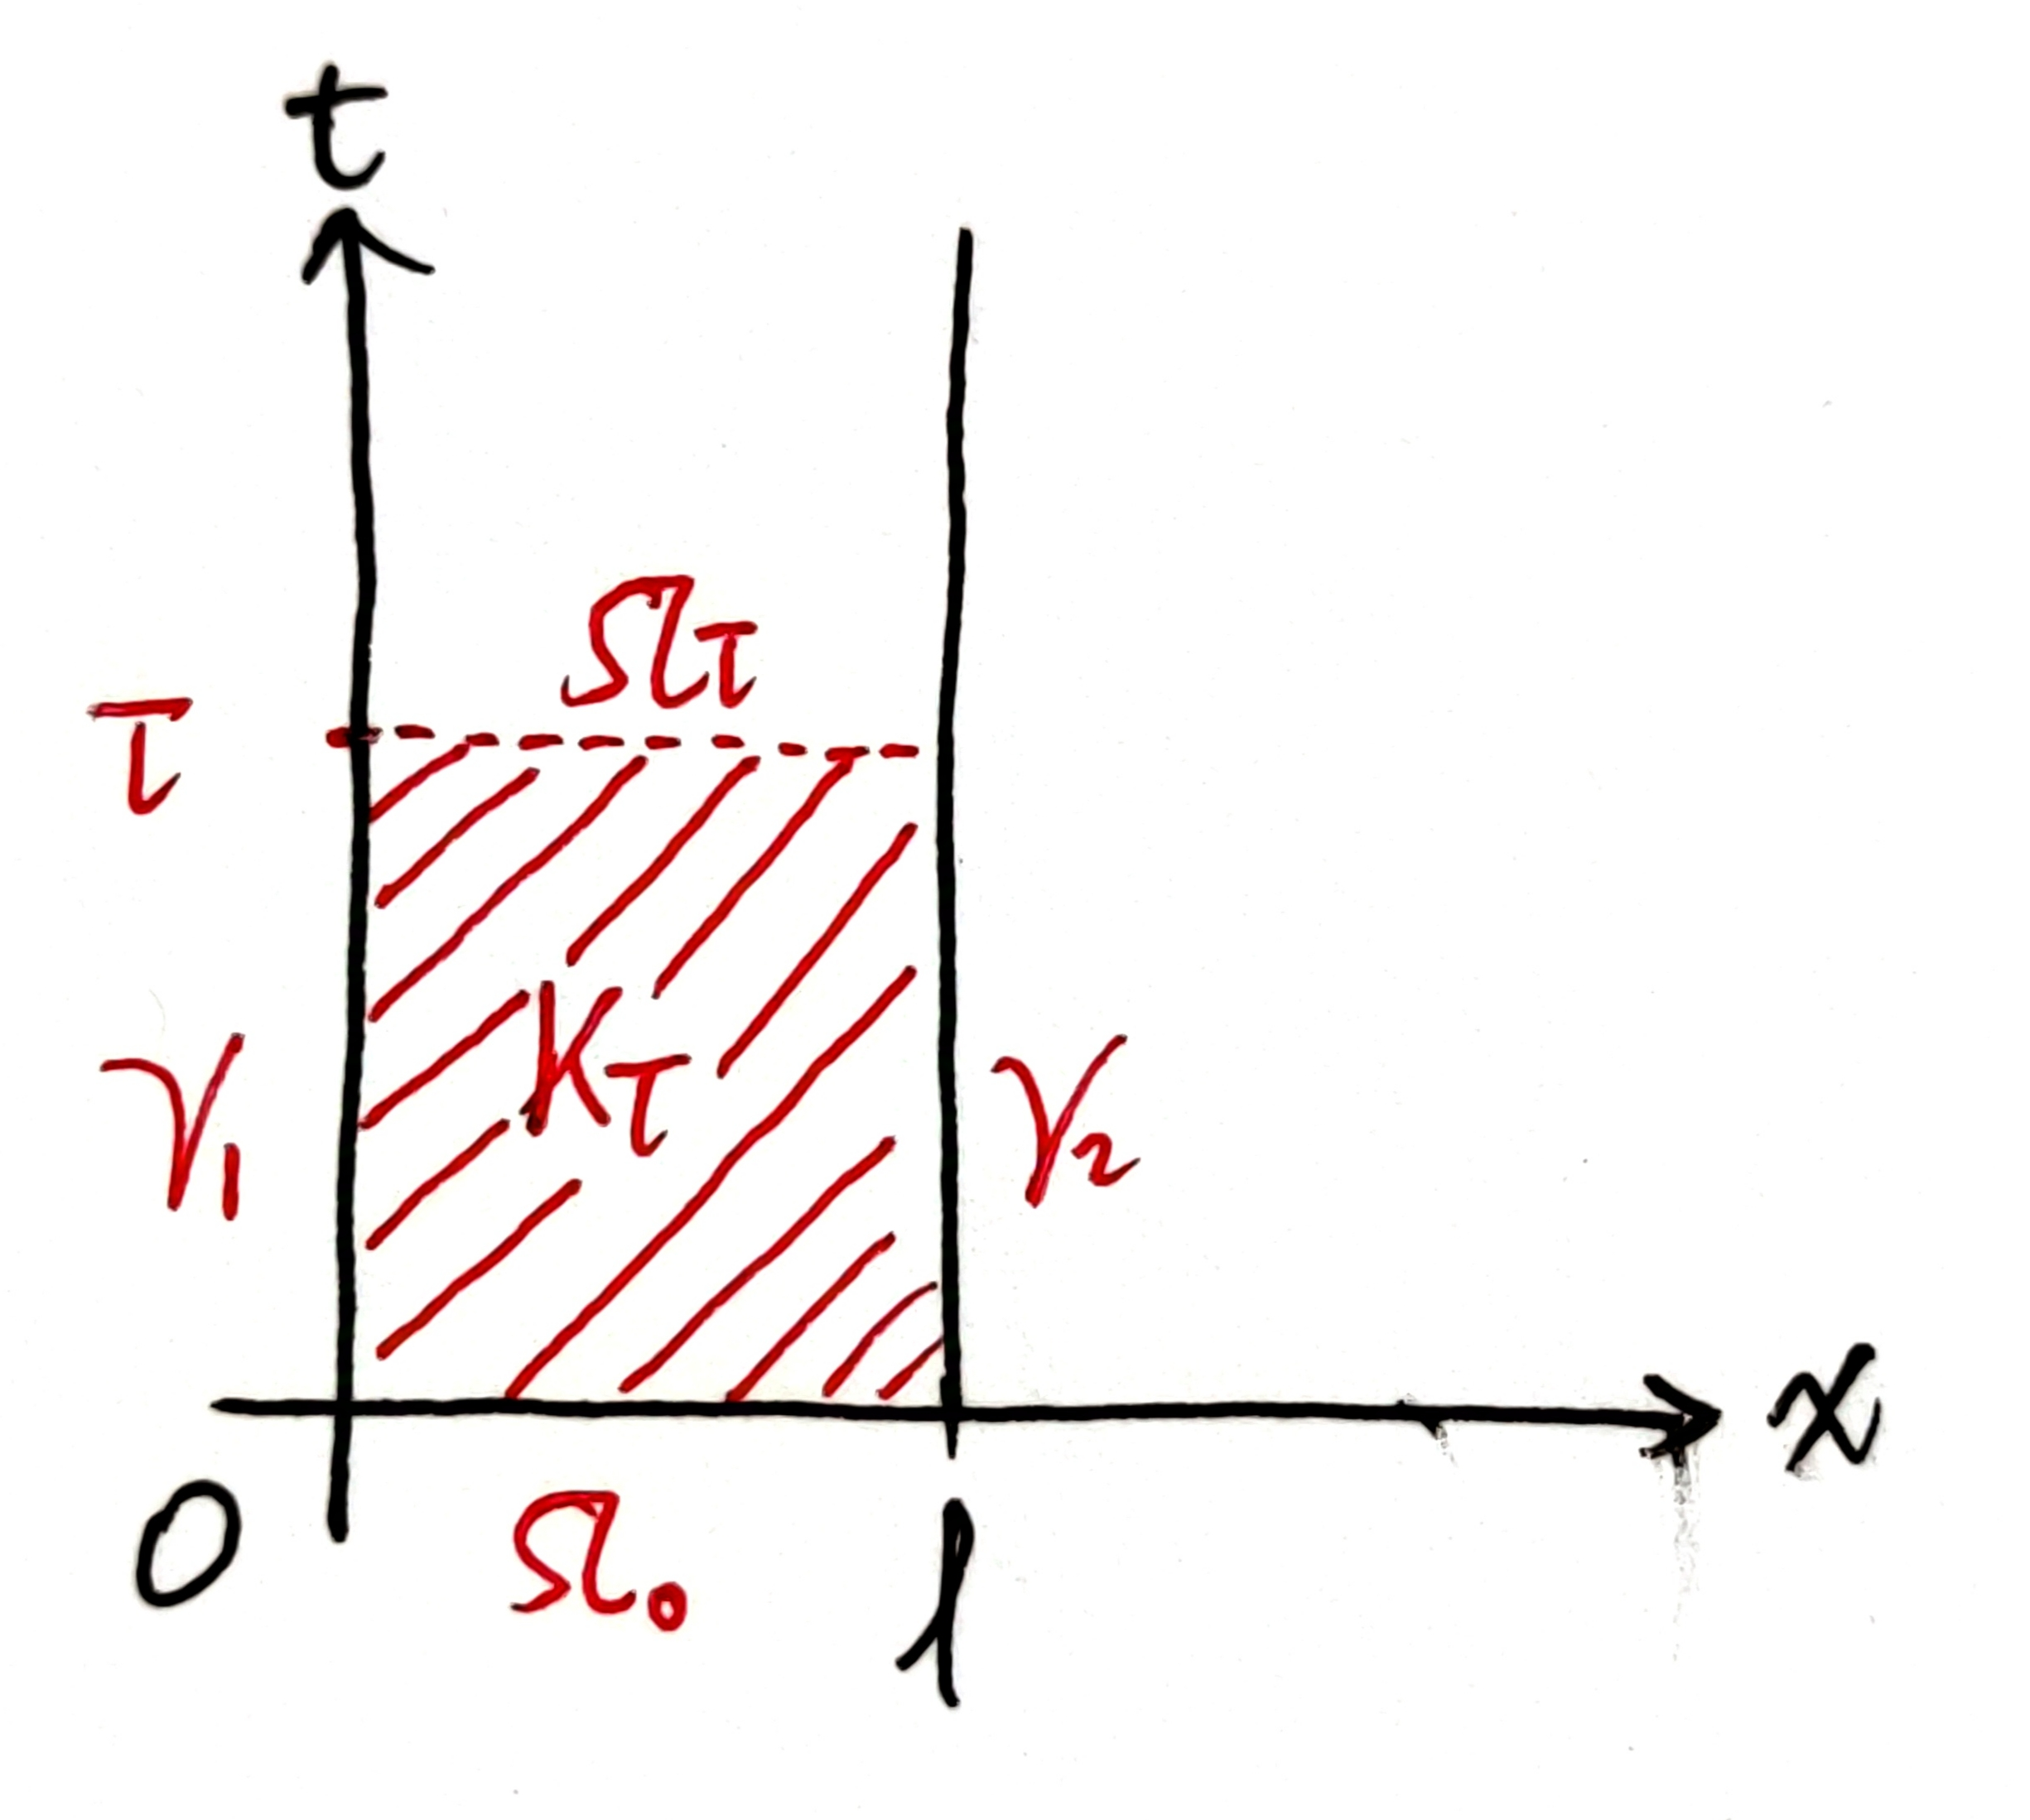
\includegraphics[width=0.28\linewidth]{figure/2.3-6}
					\caption{区域$K_\tau$ 及边界定义}
					\label{pic : 2.3-6} % 添加图像引用标签
				\end{figure}
				
				设$u(x , t)$ 为原问题 (\ref{2.17}) 的解. Then
				\begin{align*}
					\iint_{K_\tau} u_t (u_{tt} - c^2 u_{xx}) = 0
				\end{align*}
				Since
				\begin{align*}
					u_t(u_{tt} - c^2 u_{xx}) 
					&= \frac{1}{2} \frac{\partial}{\partial t} (u_{t}^2) + \frac{c^2}{2} \frac{\partial}{\partial t} (u_{x}^2) - c^2 \frac{\partial}{\partial x}(u_t u_x) \\
					&= \frac{1}{2} \frac{\partial}{\partial t}(u_{t}^2 + c^2 u_{x}^2) - c^2 \frac{\partial}{\partial x} (u_t u_x)
				\end{align*}
				Then by \textbf{Gauss-Green Theorem (Thm \ref{thm B.4.1})}, 
				\begin{align*}
					0 
					&= \iint_{K_\tau} \Big[ \frac{1}{2} \frac{\partial}{\partial t}(u_{t}^2 + c^2 u_{x}^2) - c^2 \frac{\partial}{\partial x} (u_t u_x) \Big] \\
					&= \int_{\partial K_\tau} \Big[ \frac{1}{2} (u_{t}^2 + c^2 u_{x}^2) \cdot n_t - c^2 (u_t u_x) \cdot n_x \Big] \\
					&= \int_{\Omega_0} \Big[ -\frac{1}{2} (u_{t}^2 + c^2 u_{x}^2) \Big] 
					+ \int_{\Omega_\tau} \Big[ \frac{1}{2} (u_{t}^2 + c^2 u_{x}^2) \Big] 
					+ \int_{\gamma_1} c^2 u_t u_x 
					- \int_{\gamma_2} c^2 u_t u_x
				\end{align*}
				Since $u(0 , t) = u(l , t) = 0$, then $u_t \Big|_{x = 0} = u_t \Big|_{x = l} = 0$. Thus
				\begin{align*}
					\int_{\Omega_0} \Big[ -\frac{1}{2} (u_{t}^2 + c^2 u_{x}^2) \Big] 
					+ \int_{\Omega_\tau} \Big[ \frac{1}{2} (u_{t}^2 + c^2 u_{x}^2) \Big] 
					= 0
				\end{align*}
				i.e. 
				\begin{align*}
					\int_{\Omega_\tau} (u_{t}^2 + c^2 u_{x}^2) = \int_{\Omega_0} (\psi^2 + c^2 \varphi_{x}^2) , \,\, \forall \tau > 0
				\end{align*}
				
				\newpage
				
				Suppose $u_1 \& u_2$ are both solutions of Problem (\ref{2.17}). Then 
				\begin{align*}
					\begin{cases}
						(u_1 - u_2)_{tt} - c^2 (u_1 - u_2)_{xx} = 0 , \,\, x \in (0 , l) , t > 0 \\
						(u_1 - u_2) \Big|_{t = 0} = 0 \\
						(u_1 - u_2)_t \Big|_{t = 0} = 0 \\
						(u_1 - u_2)(0 , t) = (u_1 - u_2)(l , t) = 0
					\end{cases}
				\end{align*}
				故$u_1 - u_2$ 为上述混合问题的解, 其中$\varphi = \psi = 0$. 根据混合问题的\textbf{能量不等式}, 
				\begin{align*}
					\int_{\Omega_\tau} ((u_1 - u_2)_{t}^2 + c^2 (u_1 - u_2)_{x}^2) = \int_{\Omega_0} (\psi^2 + c^2 \varphi_{x}^2) = 0 , \,\, \forall \tau > 0
				\end{align*}
				Thus
				\begin{align*}
					(u_1 - u_2)_t \equiv (u_1 - u_2)_x \equiv 0 \,\, \text{on} \, [0 , l] \times [0 , \infty)
				\end{align*}
				Hence
				\[ u_1 - u_2 \equiv C \,\, \text{for some} \,\, C \in \R \]
				Since $(u_1 - u_2) \Big|_{t = 0} = 0$, then $C = 0$. Therefore, $u_1 = u_2$. 
			\end{itemize}
		\end{proof}
	\end{thm}

\newpage

\subsection{一般的一维波动方程的分离变量法 (混合问题)}
	对于一般的一维波动方程
	
	\begin{align}
		\begin{cases}
			u_{tt} - c^2 u_{xx} = f(x , t) , \,\, x \in (0 , l) , t > 0 \\
			u \Big|_{t = 0} = \varphi(x) , \,\, x \in [0 , l]\\
			u_t \Big|_{t = 0} = \psi(x) , \,\, x \in [0 , l] \\
			\Big( -\alpha_1 u_x + \beta_1 u \Big) \Big|_{x = 0} = g(t) , \,\, t > 0 \\
			\Big( \alpha_2 u_x + \beta_2 u \Big) \Big|_{x = l} = h(t) , \,\, t > 0
		\end{cases}\label{2.21}
	\end{align}

	\vspace*{2em}

	\hspace*{-1.95em}若其满足相应的相容性条件, 则\textbf{解的存在唯一性}可类似\textbf{Thm \ref{thm 2.3.5}} 得到. 下面给出其具体运用\textbf{分离变量法}求解的步骤:
	
	\vspace*{4em}
	
	\begin{enumerate}
		\item[\textbf{Step 0}]. \underline{\textbf{Find a function $W(x , t)$}}, $\st$
		\begin{align*}
			\begin{cases}
				-\alpha_1 W_x(0 , t) + \beta_1 W(0 , t) = g(t) \\
				\alpha_2 W_x(l , t) + \beta_2 W(l , t) = h(t)
			\end{cases}
		\end{align*}
		Let $v = u - W$, 则可将$x = 0$, $x = l$ 处边界条件齐次化, i.e. 
		
		\begin{align*}
			\begin{cases}
				v_{tt} - c^2 v_{xx} = f(x , t) - (W_{tt} - c^2 W_{xx}) , \,\, x \in (0 , l) , t > 0 \\
				v \Big|_{t = 0} = \varphi(x) - W(x , 0) , \,\, x \in [0 , l]\\
				v_t \Big|_{t = 0} = \psi(x) - W_t(x , 0) , \,\, x \in [0 , l] \\
				\Big( -\alpha_1 v_x + \beta_1 v \Big) \Big|_{x = 0} = 0 , \,\, t > 0 \\
				\Big( \alpha_2 v_x + \beta_2 v \Big) \Big|_{x = l} = 0 , \,\, t > 0
			\end{cases}
		\end{align*}
		
		\vspace*{2em}
		
		\hspace*{-1.95em}故下列步骤中默认 (\ref{2.21})中$x = 0$, $x = l$ 处边界条件为$g = h = 0$. 
		
		\vspace*{1em}
		
		\item[\textbf{Step 1}]. \underline{\textbf{Sturm-Liouville Problem}}:
		\begin{align*}
			\begin{cases}
				X^{''}(x) + \lambda X(x) = 0 , \,\, x \in (0 , l) \\
				-\alpha_1 X^{'}(0) + \beta_1 X(0) = 0 \\
				\alpha_2 X^{'}(l) + \beta_2 X(l) = 0
			\end{cases}
		\end{align*}
		求解出所有的特征值$\{ \lambda_k \}_{k = 1}^{\infty}$ 及对应特征函数$\{ X_k \}_{k = 1}^{\infty}$. 
		
		\vspace*{2em}
		
		\item[\textbf{Step 2}]. \underline{\textbf{Expansion}}:\\
		根据\textbf{Sturm-Liouville问题的性质 (Thm \ref{thm 2.3.4})}, $\{ X_k \}_{k = 1}^{\infty} \subset L^2[0 , l]$ 为一组完备正交系. \\
		将$f , \varphi , \psi$ 按$\{ X_k \}_{k = 1}^{\infty}$ 展开, 
		\begin{align*}
			f(x , t) &= \sum_{k = 1}^{\infty} f_{k}(t) \cdot X_k(x) \\
			\varphi(x) &= \sum_{k = 1}^{\infty} \varphi_k \cdot X_k(x) \\
			\psi(x) &= \sum_{k = 1}^{\infty} \psi_k \cdot X_k(x)
		\end{align*}
		其中$\varphi_k , \psi_k$ 与\textbf{Thm \ref{thm 2.3.5}} 中一致, 
		\begin{align*}
			f_k(t) = \frac{\int_{0}^l f(x , t) \cdot X_k(x) \, dx}{\int_{0}^l X_{k}^2(x) \, dx}
		\end{align*}
		
		\vspace*{2em}
		
		\item[\textbf{Step 3}]. \underline{\textbf{Substitution}}:\\
		将$u(x , t) = \overset{\infty}{\underset{k = 1}{\sum}} T_K(t) \cdot X_k(x)$ 及上述展开式代入原方程 (\ref{2.21}), 结合$X_{k}^{''} = -\lambda_k X_k$, 得到
		\begin{align*}
			\begin{dcases}
				\sum_{k = 1}^{\infty} \Big( T_{k}^{''}(t) + c^2 \lambda_k T_{k}(t) \Big) \cdot X_k(x) 
				= \sum_{k = 1}^{\infty} f_k(t) \cdot X_k(x) \\
				\sum_{k = 1}^{\infty} T_k(0) \cdot X_k(x) =  \sum_{k = 1}^{\infty} \varphi_k \cdot X_k(x) \\
				\sum_{k = 1}^{\infty} T_{k}^{'}(0) \cdot X_k(x) = \sum_{k = 1}^{\infty} \psi_k \cdot X_k(x) 
			\end{dcases}
		\end{align*}
		于是得到有关$T_k(t)$ 的\textbf{ODE初值问题}:
		\begin{align*}
			\begin{cases}
				T_{k}^{''}(t) + c^2 \lambda_k T_k(t) = f_k(t) \\
				T_k(0) = \varphi_k \\
				T_{k}^{'}(0) = \psi_k
			\end{cases} , \,\, \forall k \in \N
		\end{align*}
		
		\vspace*{2em}
		
		\item[\textbf{Step 4}]. \underline{\textbf{Solve ODE}}. 对每个$k \in \N$, 求解上述$T_k(t)$, 从而得到
		\begin{align*}
			u(x , t) = \sum_{k = 1}^{\infty} T_k(t) \cdot X_k(x)
		\end{align*}
	\end{enumerate}

\newpage

\subsection{一维波动方程的广义解}
	对于任意区域上的一维波动方程
	\[ u_{tt} - c^2 u_{xx} = 0 \]
	通过求解特征线, 作变换$\xi = x + ct , \eta = x - ct$, 原方程转化为$u_{\xi\eta} = 0$, 从而解$u$ 必然满足形式
	\[ u(x , t) = F(x + ct) + G(x - ct) \]
	通过该式, 下面给出一维波动方程的解的性质. 
	
	\vspace*{2.5em}
	
	\begin{proposition}\label{prop 2.3.1}
		\textbf{[一维波动方程解的性质]}. \\
		Suppose $u(x , t)$ be a solution of the one-dimensional wave equation on any fixed region
		\[ u_{tt} - c^2 u_{xx} = 0 \]
		Then for $\forall$ 定义域内各边与特征线平行的平行四边形$ABCD$, $A(x_1 , t_1) , B(x_2 , t_2) , C(x_3 , t_3) , D(x_4 , t_4)$, $u$ satiefies 
		\[ u(x_1 , t_1) + u(x_3 , t_3) = u(x_2 , t_2) + u(x_4 , t_4) \]
		
		\begin{figure}[thbp!]
			\centering
			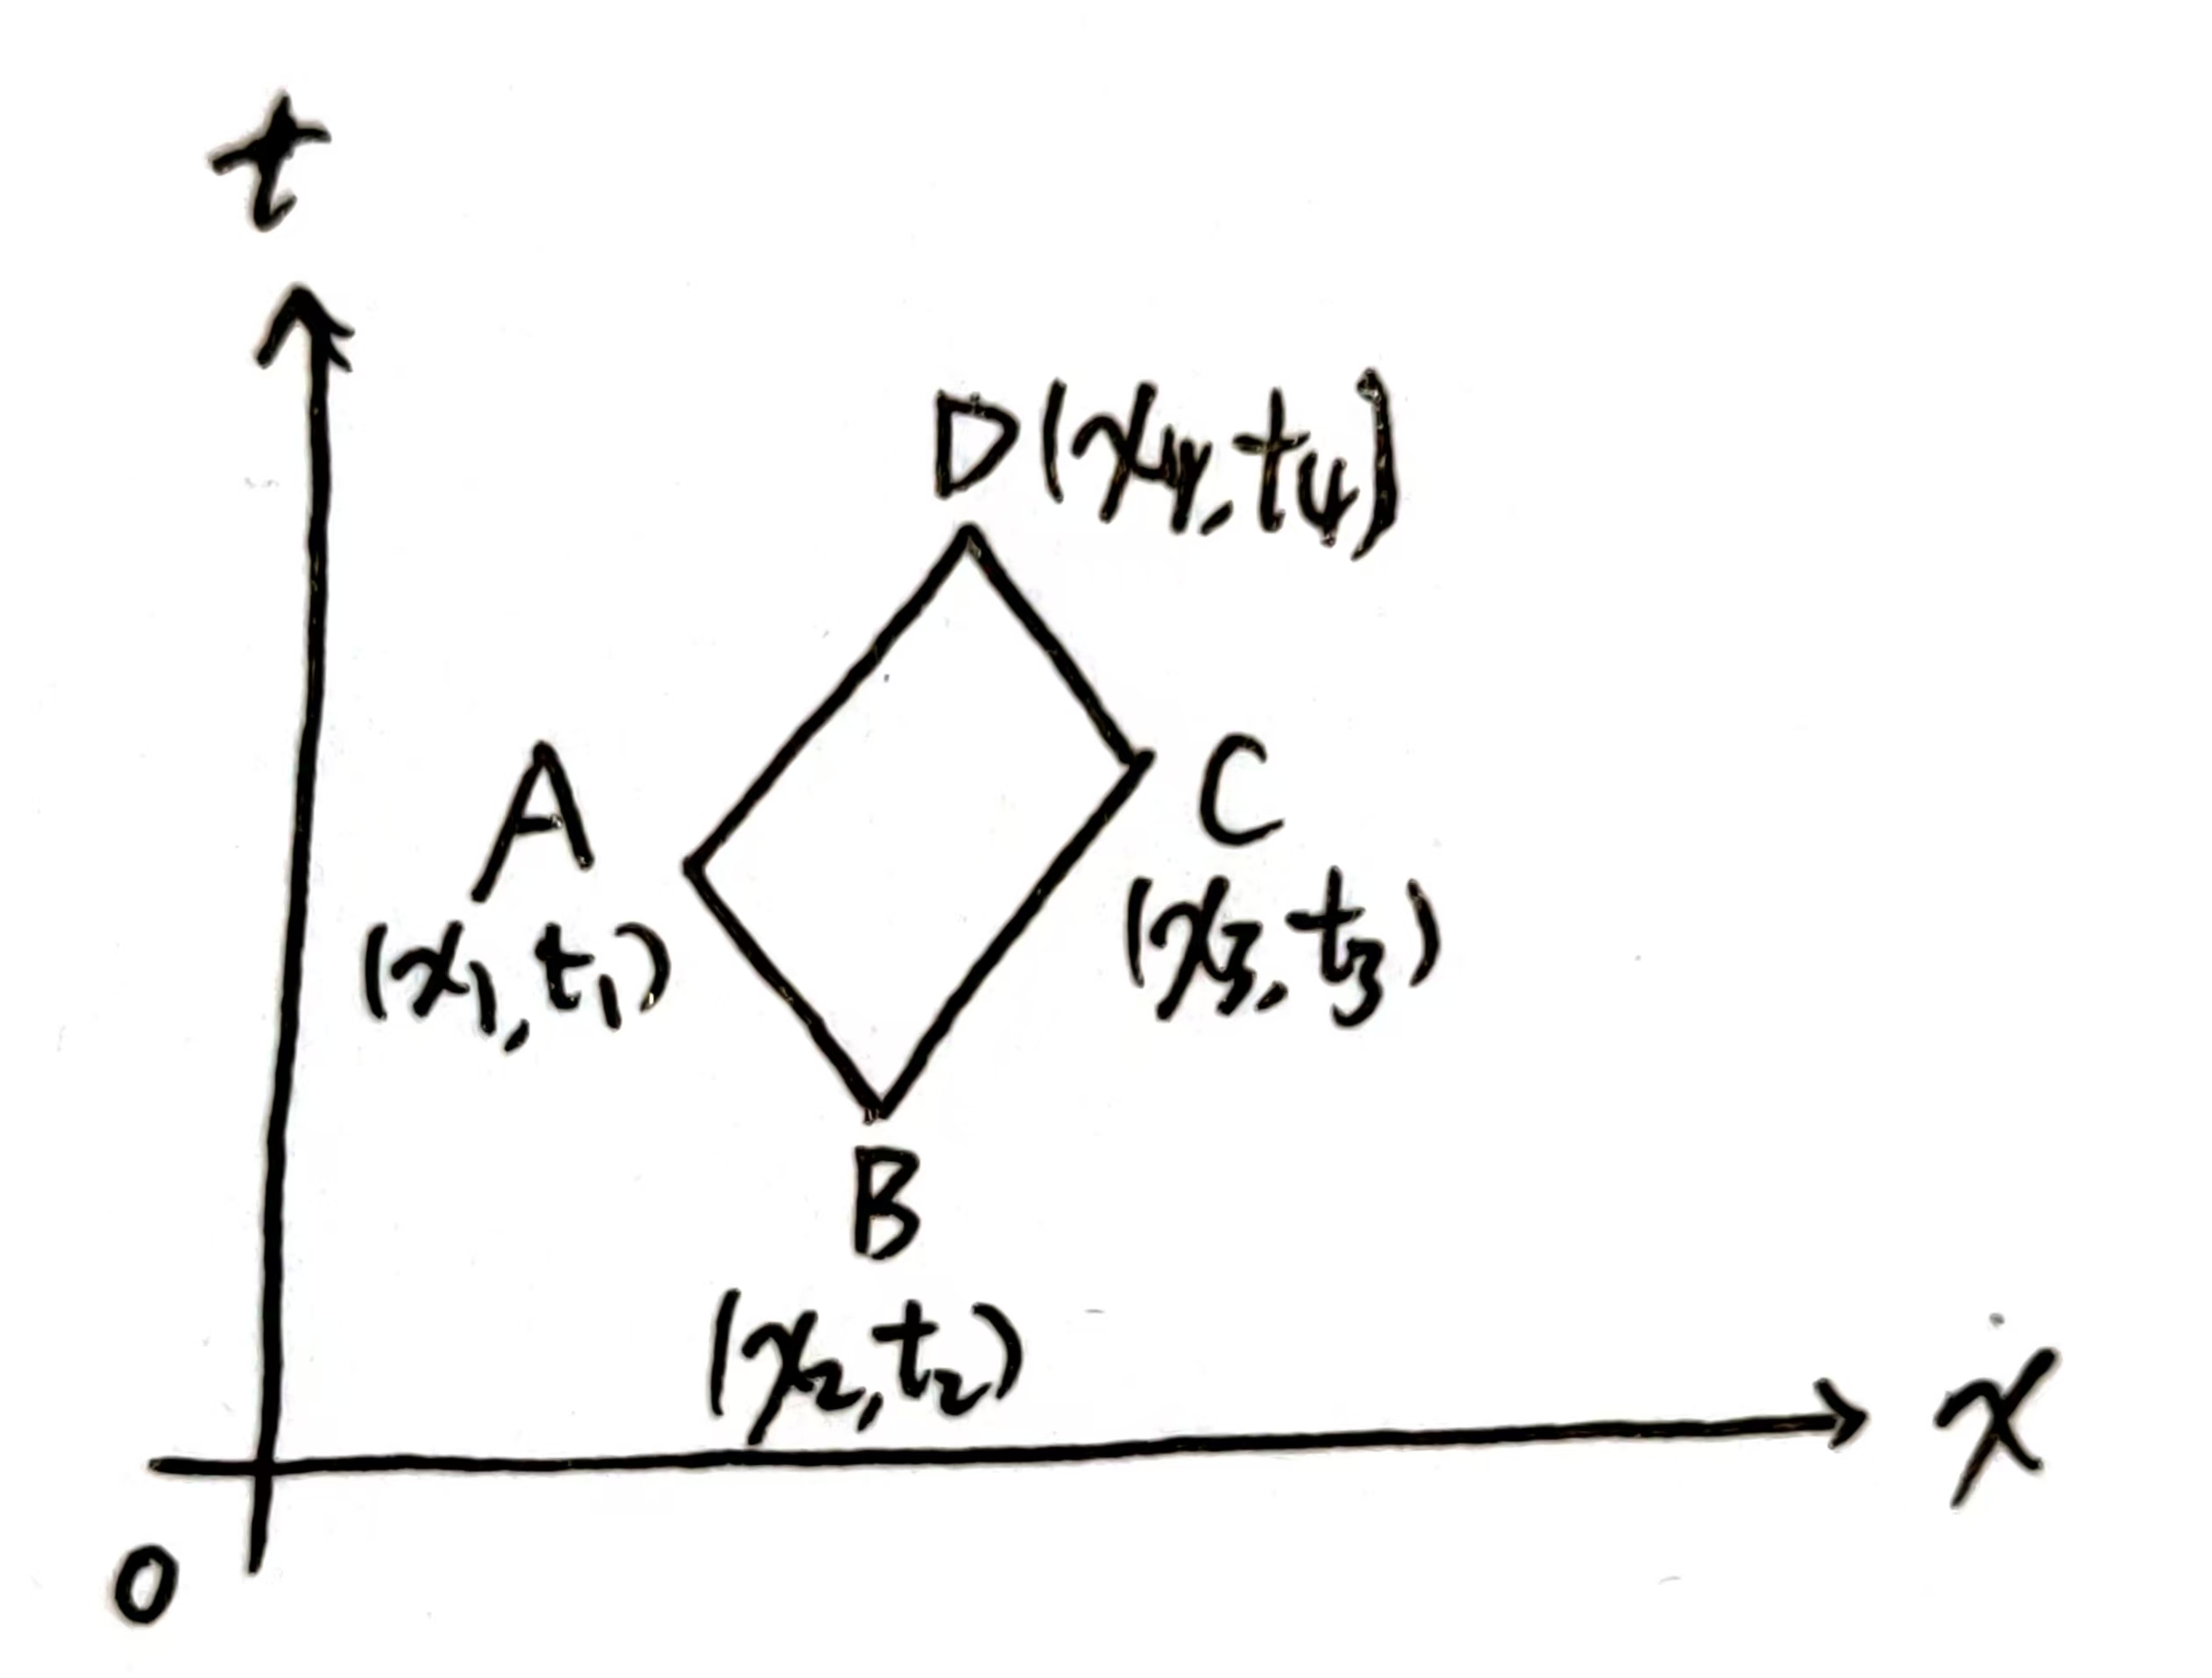
\includegraphics[width=0.3\linewidth]{figure/2.3-8}
			\caption{各边与特征线平行的平行四边形$ABCD$}
			\label{pic : 2.3-8} % 添加图像引用标签
		\end{figure}
		
		\begin{proof}
			不妨设$BD \,$ // $t$ 轴, 即$x_2 = x_4$. 设$-\dfrac{x_1 - x_2}{t_1 - t_2} = \dfrac{x_3 - x_2}{t_3 - t_2} = \dfrac{x_4 - x_1}{t_4 - t_1} = -\dfrac{x_4 - x_3}{t_4 - t_3} = c$, 有
			\[ x_1 - x_2 = -c(t_1 - t_2) , \,\, x_3 - x_2 = c(t_3 - t_2) , \,\, x_4 - x_1 = c(t_4 - t_1) \,\ x_4 - x_3 = -c(t_4 - t_3) \]
			i.e.
			\[ x_1 + ct_1 = x_2 + ct_2 , \,\, x_2 - ct_2 = x_3 - ct_3 , \,\, x_1 - ct_1 = x_4 - ct_4 , \,\, x_3 + ct_3 = x_4 + ct_4 \]
			于是
			\begin{align*}
				u(x_1 , t_1) + u(x_3 , t_3) 
				&= F(x_1 + ct_1) + G(x_1 - ct_1) + F(x_3 + ct_3) + G(x_3 - ct_3) \\
				&= F(x_2 + ct_2) + G(x_4 - ct_4) + F(x_4 + ct_4) + G(x_2 - ct_2) 
				= u(x_2 , t_2) + u(x_4 , t_4)
			\end{align*}
		\end{proof}
	\end{proposition}
	
	\newpage
	
	基于上述性质, 我们来给出一维波动方程\textbf{广义解}的定义. 
	
	\vspace*{1em}
	
	\begin{defn}\label{def 2.3.3}
		Suppose $u \in C \Big( \R \times [0 , \infty) \Big)$, $\st$ 
		\[ u(A) + u(C) = u(B) + u(D) \]
		for any parallel with characteristic curve as its sides. Then we call $u$ is a \underline{\textcolor{blue}{\textbf{generalized solution}}} of the one-dimentional wave equation 
		\[ u_{tt} - c^2 u_{xx} = 0 \]
		
		\vspace*{2em}
		
		\begin{rmk}
			一维波动方程的\textbf{广义解}的定义并不依赖于任何的初始条件及定义域, 只要求在上半平面连续, 且对任一各边与特征线平行的平行四边形满足\textbf{Prop \ref{prop 2.3.1}}即可. 下面我们会说明, 这样定义的\textbf{广义解}是对前面我们所讨论的\underline{\textcolor{blue}{\textbf{传统解 (classical solution)}}} 的推广. 
		\end{rmk}
	\end{defn}
	
	\begin{figure}[thbp!]
		\centering
		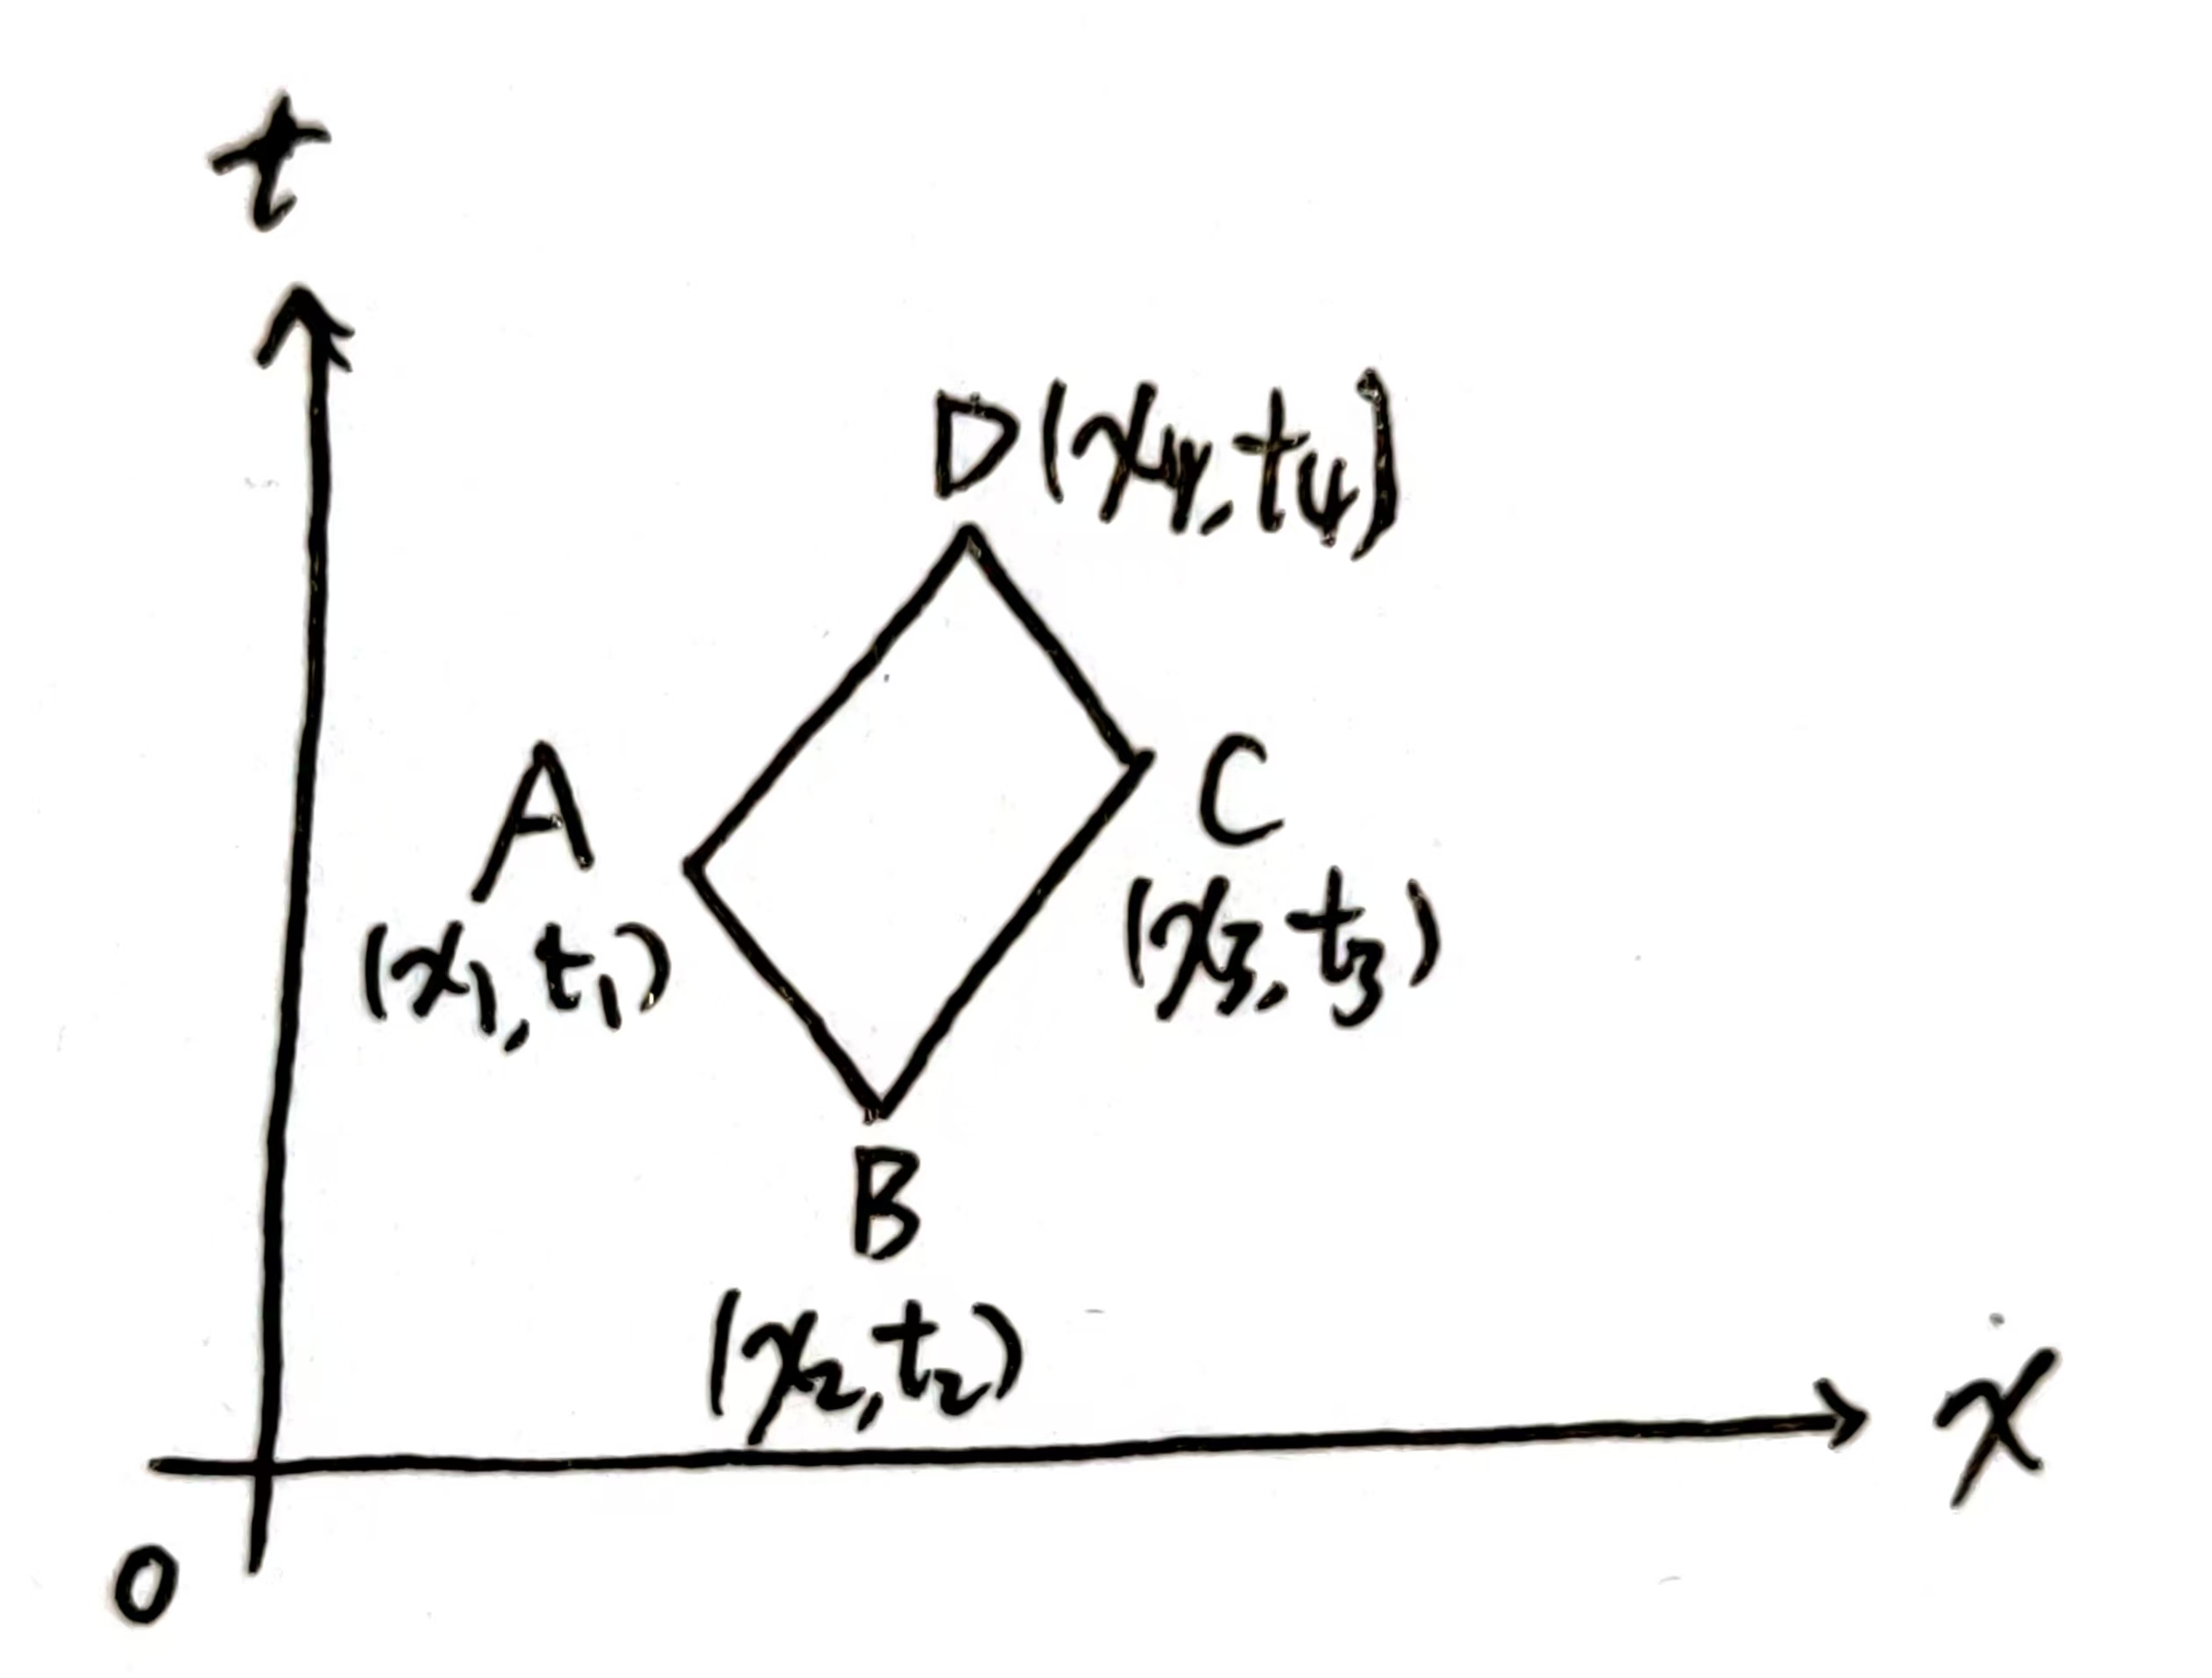
\includegraphics[width=0.3\linewidth]{figure/2.3-8}
		\caption{各边与特征线平行的平行四边形$ABCD$}
		\label{pic : 2.3-8-1} % 添加图像引用标签
	\end{figure}
	
	下面我们来说明, 这样定义的\textbf{广义解}是对\textbf{传统解}的良好推广. 
		
	\begin{figure}[thbp!]
		\centering
		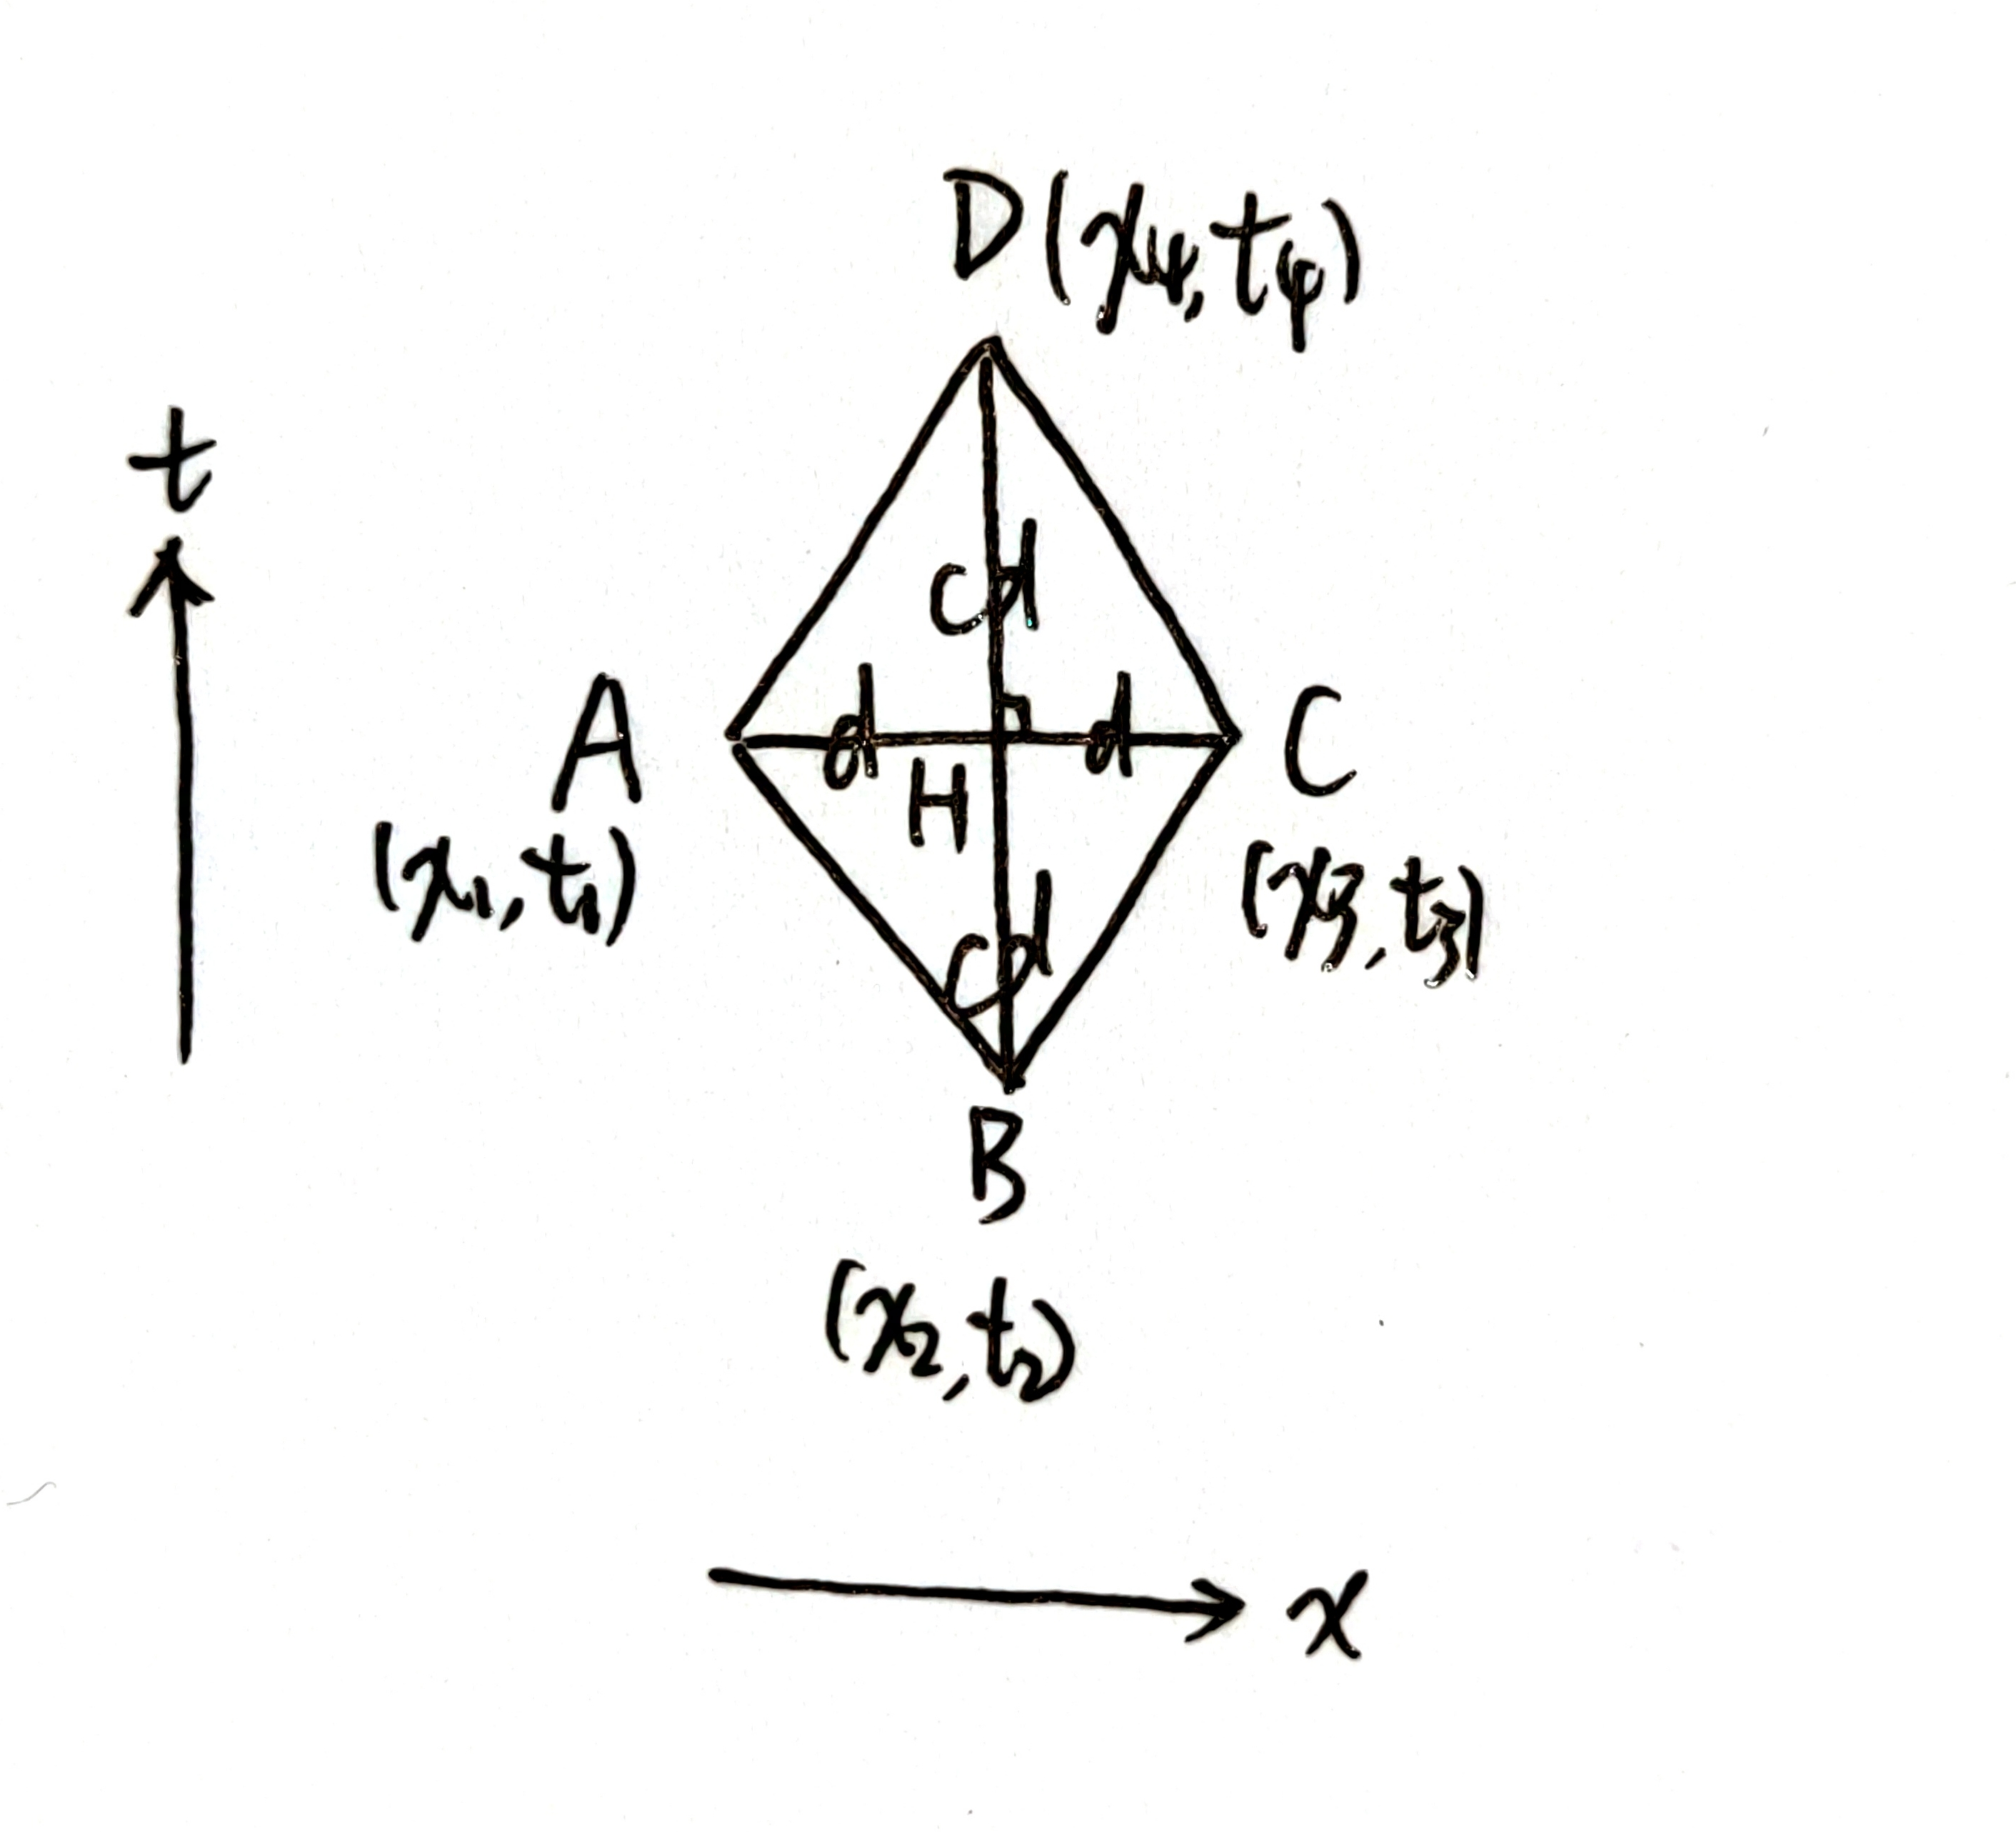
\includegraphics[width=0.35\linewidth]{figure/2.3-9}
		\caption{以$H$ 为中心的菱形$ABCD$ (各边与特征线平行, \textbf{Thm \ref{thm 2.3.6}})}
		\label{pic : 2.3-9} % 添加图像引用标签
	\end{figure}
	
	\newpage
	
	\begin{thm}\label{thm 2.3.6}
		\textbf{[一维波动方程的广义解, Well-Defined]}. \\
		对于一维波动方程$u_{tt} - c^2 u_{xx} = 0$ 的广义解, 有如下结论:
		\begin{enumerate}
			\item[(1)] Classical solutions are generalized solutions. 
			
			\item[(2)] Suppose $u$ is a generalized solution and $u \in C^2$, then $u$ is a classical solution. 
			
			\item[(3)] With boundary and initial conditions, generalized solution is unique.
		\end{enumerate}
		
		\vspace*{4em}
		
		\begin{proof}
			\textbf{Proof of (2)}:It suffices to show $u_{tt}(H) - c^2 u_{xx}(H) = 0 , \,\, \forall H \in \R \times (0 , \infty)$. \\
			Fix $\forall H \in \R \times (0 , \infty)$. Take 以$H$ 为中心的菱形$ABCD$, $\st$ $AC \,$ // x轴, $BD \,$ // t轴.  \\
			$A(x_1 , t_1) , B(x_2 , t_2) , C(x_3 , t_3) , D(x_4 , t_4)$. \\
			Since $ABCD$ 各边平行于特征线, then suppose 
			\[ \left| HA \right| = \left| HC \right| = d > 0 , \,\, \left| HB \right| = \left| HD \right| = cd \]
			By \textbf{Taylor's Formula}, 
			\begin{align*}
				u(x_1 , t_1) 
				= u(H) + \nabla u(H) \cdot \overrightarrow{HA} + \frac{1}{2} \overrightarrow{HA}^T 
				\left. 
				\begin{pmatrix*}
					u_{xx} &u_{xt} \\
					u_{xt} &u_{tt}
				\end{pmatrix*} 
				\right|_{H} \overrightarrow{HA} + \circ(d^2) 
			\end{align*}
			同理可得到$u(x_i , t_i) , \,\, \forall i = 1 \sim 4$ 在$H$ 点的展开式. Then \\
			By $u(A) + u(C) = u(B) + u(D)$, with $\overrightarrow{HA} + \overrightarrow{HC} = \overrightarrow{HB} + \overrightarrow{HD} = \vec{0}$, we have
			\begin{align*}
				\overrightarrow{HA}^T 
				\left. 
				\begin{pmatrix*}
					u_{xx} &u_{xt} \\
					u_{xt} &u_{tt}
				\end{pmatrix*} 
				\right|_{H} \overrightarrow{HA} + 
				\overrightarrow{HC}^T 
				\left. 
				\begin{pmatrix*}
					u_{xx} &u_{xt} \\
					u_{xt} &u_{tt}
				\end{pmatrix*} 
				\right|_{H} \overrightarrow{HC} 
				= 
				\overrightarrow{HB}^T 
				\left. 
				\begin{pmatrix*}
					u_{xx} &u_{xt} \\
					u_{xt} &u_{tt}
				\end{pmatrix*} 
				\right|_{H} \overrightarrow{HB} + 
				\overrightarrow{HD}^T 
				\left. 
				\begin{pmatrix*}
					u_{xx} &u_{xt} \\
					u_{xt} &u_{tt}
				\end{pmatrix*} 
				\right|_{H} \overrightarrow{HD} + \circ(d^2)
			\end{align*}
			Since $AC \,$ // x轴, $BD \,$ // t轴, then
			\[ \overrightarrow{HA} = (-d , 0) , \,\, \overrightarrow{HC} = (d , 0) , \,\, \overrightarrow{HB} = (0 , -cd) , \,\, \overrightarrow{HD} = (0 , cd) \]
			代入上式, 得到
			\[ 2d^2 u_{tt}(H) = 2c^2 d^2 u_{xx}(H) + \circ(d^2) \]
			i.e. 
			\[ u_{tt}(H) - c^2 u_{xx}(H) = \frac{\circ(d^2)}{d^2} \]
			Letting $d \to 0^+$, we have proved $u_{tt} - c^2 u_{xx} = 0$. 
		\end{proof}
	\end{thm}
	
	


	%  ############################
	\ifx\allfiles\undefined
\end{document}
\fi